%% Copyright 2019-2024 Elsevier Ltd
%% 
%% This file is part of the 'CAS Bundle'.
%% --------------------------------------
%% 
%% It may be distributed under the conditions of the LaTeX Project Public
%% License, either version 1.3c of this license or (at your option) any
%% later version.  The latest version of this license is in
%%    http://www.latex-project.org/lppl.txt
%% and version 1.3c or later is part of all distributions of LaTeX
%% version 1999/12/01 or later.
%% 
%% The list of all files belonging to the 'CAS Bundle' is
%% given in the file `manifest.txt'.
%% 
%% Template article for cas-sc documentclass for 
%% double column output.

\documentclass[a4paper,fleqn]{cas-sc}

% If the frontmatter runs over more than one page
% use the longmktitle option.

%\documentclass[a4paper,fleqn,longmktitle]{cas-sc}

% \usepackage[numbers]{natbib}
\usepackage[authoryear]{natbib}
% \usepackage[authoryear,longnamesfirst]{natbib}

\usepackage[utf8]{inputenc}
\usepackage[cjk]{kotex} % for writing korean characters
\CJKscale{1} % korean font scale setting
\graphicspath{{figs/}} % image base directory
\usepackage{subcaption}
\usepackage{tabularx}
\usepackage{siunitx}
\usepackage{graphicx}
\graphicspath{{figure/}}
\usepackage{float}
\usepackage{placeins}
\usepackage{cleveref}

%%%Author macros
% \def\tsc#1{\csdef{#1}{\textsc{\lowercase{#1}}\xspace}}
% \tsc{WGM}
% \tsc{QE}

% Uncomment and use as if needed
\newdefinition{definition}{Definition}
%\newtheorem{theorem}{Theorem}
%\newtheorem{lemma}[theorem]{Lemma}
%\newdefinition{rmk}{Remark}
%\newproof{pf}{Proof}
%\newproof{pot}{Proof of Theorem \ref{thm}}

\begin{document}
\let\WriteBookmarks\relax


\def\floatpagepagefraction{1}
\def\textpagefraction{.001}

% Short title
\shorttitle{Efficient Knowledge Expansion Strategies in Fake News Detection}    

% Short author
% \shortauthors{}  

% Main title of the paper
\title [mode = title]{Efficient Knowledge Expansion Strategies in Fake News Detection}

% author 1
\author[1]{Jeongwook Lee}[orcid=0000-0002-0100-0390]
\ead{jwlee@g.kmou.ac.kr} % Email id of the first author
\credit{Conceptualization, Methodology, Validation, Writing - original draft}

% author 2
\author[1]{Jae-Hoon Kim}[orcid=0000-0001-8655-2591]
\ead{jhoon@kmou.ac.kr}
\credit{Writing – review \& editing, Supervision}
\cormark[1]
\cortext[1]{Corresponding author} % Corresponding author text

% Address/affiliation
\affiliation[1]{organization={Department of Computer Engineering and Interdisciplinary Major of Maritime AI Convergence, Korea Maritime and Ocean University},
            addressline={727, Taejong-ro, Yeongdo-gu}, 
            city={Busan},
%          citysep={}, % Uncomment if no comma needed between city and postcode
            postcode={49112}, 
            % state={},
            country={S.Korea}}


% For a title note without a number/mark
%\nonumnote{}

% Here goes the abstract
\begin{abstract}
ㅇㅇ
%학위논문은 대규모 언어모델(LLM)의 Fine-tuning 과정에서 발생하는 하드웨어 자원 소모 문제를 극복하기 위해, 문장 단위 분류 모델과 관계 인식 파인튜닝(relation-aware fine-tuning)이라 명명한 새로운 학습 전략을 제안하며, 적용 도메인으로는 fake news detection을 선정하였다. 본 연구는 두 단계로 수행되었다. 첫 번째 단계에서는 COVID-19 가짜뉴스에 특화된 한국어 데이터셋을 구축하고, KoCharELECTRA 기반 임베딩과 BiLSTM 분류기를 결합한 문장 단위 탐지 모델을 개발하였다. 기존 [CLS] 토큰 기반 분류 모델과 달리, 제안된 모델은 BiLSTM 구조를 도입하여 음절 수준의 맥락 정보를 효과적으로 반영한다. 특히 [CLS] 토큰을 BiLSTM의 은닉 상태와 셀 상태 초기값으로 활용함으로써, 문장의 의미적 흐름을 정교하게 모델링할 수 있도록 설계하였다. 또한 대규모 범용 가짜뉴스 코퍼스를 사전학습한 후, COVID-19 특화 데이터로 추가 파인튜닝을 수행하여 도메인 적응성을 강화하였다. 두 번째 단계에서는 기존 모델 편집 기법의 한계를 극복하기 위해 관계 인식 파인튜닝 프레임워크를 제안하였다. 본 프레임워크는 RAG의 FAISS 기반 의미 검색, Cross Encoder 기반 재랭킹, 자연어 추론(NLI) 기반 관계 분류를 결합하여, 쿼리와 검색된 문장 간의 논리적 관계(함의, 모순, 중립)에 따라 선택적으로 파인튜닝을 적용한다. 실험 결과, 제안된 방법은 기존 파인튜닝과 유사한 정확도를 유지하면서도 locality, 편집 안정성, 일반성, 지식 일반화 측면에서 크게 향상된 성능을 보였다. 특히 인코더 전체를 조정하지 않고 인코더 내 MLP 계층만을 갱신하도록 제한한 결과, 성능 저하 없이 학습 효율성을 크게 개선할 수 있었으며, 이는 자원 제약 환경에서의 실용성을 입증한다. 결론적으로, 본 논문은 데이터 중심의 문장 분류에서 NLI 기반 지식 편집으로 전환하는 새로운 학습 패러다임을 제시한다. 제안된 방법은 가짜뉴스 탐지 성능을 고도화할 뿐 아니라, 지속적인 지식 정제를 통해 신뢰성과 적응성을 갖춘 AI 시스템 구축의 견고한 기반을 제공한다. 
\end{abstract}

% Use if graphical abstract is present
%\begin{graphicalabstract}
%\includegraphics{}
%\end{graphicalabstract}


% Keywords
% Each keyword is seperated by \sep
\begin{keywords}
 Fake news detection\sep
 Knowledge based model editing\sep
 Natural language inference\sep
 Selective fine-tuning\sep
 RNN\sep
\end{keywords}

\maketitle

%============================================================%
% Introduction						     %
%============================================================%
\section{Introduction}

오늘날 대규모 언어 모델(Large Language Models, LLMs)의 발전은 자연어 처리 기술의 패러다임을 근본적으로 변화시켰다. 
수십억 개 이상의 파라미터를 가진 LLM은 질의응답, 요약, 분류, 생성 등 다양한 태스크에서 사람 수준의 성능을 보이며, 산업과 공공 분야에 이르기까지 폭넓게 활용되고 있다. 
그러나 이러한 놀라운 성과 뒤에는 여전히 해결되지 않은 핵심적인 기술 과제가 존재한다. 
이는 모델이 새로운 정보나 지식 변화에 얼마나 신속하고 효율적으로 적응할 수 있는지를 평가하고, 그 과정에서 발생하는 기술적 제약을 해결하는 것이다.
기존의 fine-tuning 방식은 새로운 데이터를 모델에 반영하는 가장 직접적인 방법으로 널리 사용되어 왔다. 
하지만 LLM의 파라미터 수가 기하급수적으로 증가함에 따라, 전체 모델을 다시 학습하는 방식은 막대한 시간, GPU 메모리, 연산 비용을 요구하게 된다. 
특히 실시간성이 요구되는 서비스나 지속적으로 데이터가 유입되는 환경에서는 전체 모델을 반복적으로 재학습하는 방식은 유지보수 측면에서도 현실적이지 않다. 
이러한 문제를 해결하기 위해, 최근에는 fULL fine-tuning을 수행하지 않으면서도 최신 정보를 모델의 출력에 반영할 수 있는 다양한 접근이 시도되어 왔다. 
대표적인 예로는 Retrieval-Augmented Generation (RAG), Continual Learning, Information Injection (e.g., Zero-shot, Few-shot, In-context Learning), Knowledge-Based Editing (KME) 등이 있다.
RAG는 외부 지식을 검색해 조건으로 활용함으로써 유연한 지식 반영이 가능하지만, 생성 결과의 정합성을 보장하기 어렵고, 논리적으로 일관되지 않은 응답을 생성할 수 있다. 
Continual learning은 기존 지식을 유지하면서도 순차적으로 학습이 가능하다는 점에서 이상적인 방법으로 보이지만, 실제로는 catastrophic forgetting 문제와 데이터 순서에 민감하다는 심각한 제약이 존재한다. 
Zero-shot이나 Few-shot prompting 등은 빠르고 유연하지만, reasoning이나 정합성이 요구되는 작업에서는 불안정한 성능을 보이는 경우가 많다.
adaptive layer 기반 학습 기법(예: LoRA)  이 방식은 파라미터 전체가 아닌 저차원의 랭크 공간에만 변화를 가함으로써, 계산 자원은 절감하면서도 fine-tuning 효과를 얻을 수 있게 한다.
새로운 정보를 모델에 반영하는 작업은 여전히 어려운 문제로 남아 있으며, 단순한 파인튜닝 또는 프롬프트 기반 접근만으로는 불충분하다.
이러한 문제는 특히 가짜 뉴스 탐지(Fake News Detection)와 같은 태스크에서 더 치명적이다. 
이 분야는 시의성 있는 정보가 핵심이며, 시간에 따라 사실 여부가 바뀌거나, 상반되는 정보가 등장하는 경우가 많다. 
최근에는 소셜 미디어(SNS)나 인터넷을 통해 Hallucination이 포함된 정보, 또는 빠르게 생성되는 새로운 데이터가 폭발적으로 증가하고 있다. 
COVID-19와 같은 급변하는 이슈에 대해 모델이 정합성 있는 판단을 내리기 위해서는, 이러한 최신 정보의 반영이 필수적이다. 
비록 COVID-19의 유행은 전 세계적으로 어느 정도 완화되었지만, 향후 유사한 보건 위기가 재발할 가능성은 여전히 존재하며, 이로 인해 COVID-19 가짜 뉴스 탐지에 대한 연구는 여전히 활발히 진행되고 있다.
따라서 모델은 끊임없이 변화하는 정보에 적응하면서도, 기존에 학습한 지식을 유지할 수 있어야 한다. 
이러한 배경 속에서 최근 주목받고 있는 방법이 바로 Knowledge-Based Editing (KME)이다.
%KME는 대규모 언어 모델(LLM)의 지식 기반을 효율적으로 수정하는 방법론으로, 전체 모델을 재학습하지 않고도 모델의 출력을 특정 방식으로 변경할 수 있게 한다. 
%이는 LLM의 응답 신뢰성 향상, 최신 정보 반영, 유해한 정보 제거 등의 실질적인 요구에 대응하는 방식으로 최근 주목받고 있다.
%KME는 인간의 학습 단계를 참고하여 세 가지 위상으로 나눌 수 있다: Recognition, Association, Mastery【148†A Comprehensive Study】. Recognition Phase는 외부 지식을 검색하거나 삽입해 모델이 새로운 정보를 인식하게 만드는 단계로, RAG나 In-context Learning이 대표적이다. Association Phase에서는 LoRA나 adapter와 같은 방식으로 모델의 표현에 새로운 지식을 연결하며, Mastery Phase에서는 기존 파라미터를 직접 수정하여 지식을 완전히 내재화한다. ROME, MEMIT, MEND 등이 대표적인 Mastery 기반 기법이다.

%이러한 KME 기법들은 다음과 같은 지표로 평가된다: (1) Edit Success – 목표 지식 수정의 정확도, (2) Portability – 유사 질의에도 수정 효과가 유지되는가, (3) Locality – 비관련 지식에는 영향이 없는가, (4) Fluency – 출력 문장의 자연성 유지.

하지만, 현재 제안된 ROME, MEMIT과 같은 기법들은 대부분 단일 문장에 대한 단순한 지식 삽입 방식에 국한되며, 기존의 잘못된 정보를 삭제하거나 정정하는 기능이 부재하다. 
이는 모델 내부의 지식 충돌을 유발할 수 있으며, 오히려 모델의 일관성과 신뢰도를 떨어뜨릴 가능성이 있다. 또한 복잡한 다중 문장 추론이나 문맥 기반 관계성을 반영하지 못하는 한계가 있다.

- 수정 대상 추출의 어려움

- 복잡한 다중 문장 추론의 부재

- 논리 관계 무시에 따른 비정합성 문제

이처럼 기존의 다양한 접근 방식들은 각기 유용한 특성을 가지고 있지만, "새로운 정보가 기존 지식과 어떤 관계에 있는지를 평가하고, 그 관계에 따라 모델을 선택적으로 fine-tuning할 수 있는 구조"는 아직 명확히 제시되지 않았다.
본 논문은 바로 이 지점에 주목하여, Knowledge-Based Editing의 개념을 확장한 Relation-aware Fine-tuning이라는 새로운 학습 전략을 제안한다. 
이 접근은 RAG, Continual Learning, Prompt-based Learning, Knowledge Editing의 장점을 통합하면서도, 그들의 구조적 한계를 보완할 수 있는 포괄적인 접근 방식이다.
Relation-aware Fine-tuning의 핵심 아이디어는 다음과 같다:
새롭게 수집된 문장이나 정보가 모델의 기존 출력 결과와 어떤 논리적 관계(Entailment, Contradiction, Neutral)를 갖는지를 먼저 평가한다.
이 관계 평가는 자연어 추론(Natural Language Inference, NLI) 기반의 구조를 사용하여 자동으로 수행된다.
특히, 새로운 정보가 기존 예측과 모순되는 경우(Contradiction)에만 fine-tuning을 수행하고, **포함(Entailment)**의 경우는 유지, **중립(Neutral)**인 경우는 별도의 중립 데이터로 보존하여 필요 시 활용하는 방식이다.

또한 본 연구에서는 이 판단 과정에 있어 모델의 confidence (softmax 기반 신뢰도)를 함께 고려한다. 
Confidence가 일정 임계값 이상(예: τ ≥ 0.7)일 때에만 관계 평가를 수행하고, 그렇지 않은 경우는 update를 보류하거나 중립 데이터로 분류함으로써, 불확실한 판단에 근거한 과도한 업데이트나 노이즈 반영을 방지한다.


기존 연구들은 대개 Locality 또는 Generality 중 하나에 초점을 맞추는 경향이 있다. 예를 들어 ROME은 편집의 국지적 영향 최소화를 중시하며, 반면 MEMIT은 다수의 지식을 한 번에 수정하여 범용성을 확보하는 데 주력한다. 그러나 이들 접근은 두 가지 목표 사이의 균형을 충분히 고려하지 못한다는 한계가 있다.
본 연구에서 제안하는 Relation-aware Fine-tuning은 생성된 응답과 검색된 문장 간의 논리 관계를 정밀하게 판단하고, 해당 관계에 따라 선택적으로 fine-tuning을 수행함으로써, Locality와 Generality를 동시에 만족할 수 있도록 설계되었다.

이러한 Relation-aware Fine-tuning 전략은 기존 접근 방식들에 비해 다음과 같은 강력한 장점을 제공한다:
\begin{itemize}
	\item{\textbf{1}:
	전체 데이터를 재학습하지 않고도 논리적 관계에 기반한 최소한의 업데이트로 최신성 확보}

	\item{\textbf{2}:
	기존 지식의 유지와 새로운 지식 반영의 균형 확보}

	\item{\textbf{3}:
	자원 및 연산 비용의 절감, 특히 대규모 모델에서의 효율적인 유지 관리 가능}

	\item{\textbf{4}:
	데이터의 정합성 확보, 검색 기반이나 프롬프트 기반 방식에서 발생하는 논리적 비일관성 문제 최소화}
\end{itemize}

본 연구는 이러한 Relation-aware Fine-tuning 전략의 가능성을 검증하기 위해, 이를 COVID-19 관련 가짜 뉴스 탐지 태스크에 적용하였다. 
COVID-19는 정보가 빠르게 변화하고, 다양한 시점에서 상반되는 정보들이 등장하기 때문에, 가짜 뉴스 탐지 모델은 지속적인 업데이트가 요구된다. 
하지만 모든 뉴스를 그대로 모델에 학습시키는 것은 비효율적이며, 오히려 모델의 기준을 혼란스럽게 만들 수 있다. 
본 연구에서는 새로운 뉴스 문장이 기존 예측과 모순될 때만 fine-tuning을 수행하도록 하여, 최소한의 학습으로 최대의 정보 반영 효과를 얻었으며, 전체 데이터를 학습시키지 않고도 기존 방법에 준하거나 더 나은 성능을 달성할 수 있음을 실험을 통해 확인하였다.
결과적으로, 본 논문은 지식 기반 편집, RAG, 지속 학습 등 기존 방법의 한계를 보완하면서, 실제 응용 가능한 효율적이고 유연한 새로운 fine-tuning 패러다임을 제시한다. 
제안된 Relation-aware Fine-tuning은 단지 COVID-19나 fake news detection에 국한된 것이 아니라, 정보 변화가 빠르고 정합성이 중요한 모든 도메인에서 일반화 가능한 전략으로 활용될 수 있다.
특정 layer를 찾아 fine-tuning하는 방법이 아닌 mlp layer만-- 실험을 통해서
모델의 성능은 ~~~~~~~~~~~
논문의 구조는 ~~~~~~~~~~~~~~;

%2022년 아스트라제네카는 맞아도 되는 백신 현재는 안된다.

%============================================================%
% Related works						     %
%============================================================%
\section{Related works}
\subsection{fake news detection}
가짜 뉴스에 따른 피해가 급증함에 따라 가짜 뉴스를 탐지하기 위한 시도가 활발하게 진행되고 있다d. 
기존의 해외 연구는 고전적인 기계학습 방법인 Classification tree 예측이나 SVM등을 사용한 모델로 문서의 여러 가지 자질을 추출하고 가짜 뉴스를 탐지한다. 
다른 연구에서는 뉴스를 공유하는 사용자와 컨텐츠의 관계를 추론하기 위해 그래프 기반 모델을 사용했다. 트위터나 페이스북과 같은 빅테크 기업에서는 딥러닝 알고리즘을 사용하여 가짜 뉴스 탐지 모델의 성능을 크게 향상했다. 
국내에서도 가짜 뉴스 탐지 분야에서 여러 연구가 진행되고 있다. 
국가차원에서는 국내선거관리위원회에서 가짜 뉴스를 정치적 목적으로 사용하는 경우를 막기 위해 비방 흑색선전 전담 TF팀을 구성하여 운영해왔으며 과학기술정보통신부에서는 인공지능 RD 챌린지를 개최하여 인공지능 기술을 사용한 가짜 뉴스 탐지 연구를 하고 있다. 
또한, 민간차원에서 팩트체크 사이트를 운영함에 따라 가짜 뉴스 탐지 데이터를 구축할 수 있게 되었다. 
데이터를 정제하여 이를 기계학습 및 딥러닝에 적용하는 연구가 진행되어 왔다.
가짜 뉴스 탐지는 여러 뉴스 카테고리에 대해 연구되어왔다. 
특정 카테고리에 대한 가짜뉴스 탐지는 데이터 부족으로 영어로 작성된 뉴스들을 중심으로 수행되어 왔다. 특히 코로나-19가짜 뉴스 탐지는 주로 해외에서 연구되고 있다. 팩트체크 사이트로부터 기사를 수집하여 BERT 기반의 모델로 코로나-19데이터셋을 구축했다. 소셜 미디어 네트워크인 트위터에서 전파되는 코로나-19관련 가짜 뉴스 탐지를 위해 Hand-crafted features를 추출하여 가짜 뉴스를 탐지했다. 하지만 코로나가 몇 년 동안 지속되고 있음에도 국내에서는 한국어로 작성된 코로나-19관련 뉴스 데이터부족으로 코로나-19가짜 뉴스 탐지 연구가 제대로 이루어지지 않고 있다.

- COVID-19 및 일반 도메인의 가짜 뉴스 탐지 방식
- 한국어 기반 가짜 뉴스 연구
- 최신 뉴스에 민감하다.
- llm의 등장으로 새로운 fine-tuning방법 하드웨어 자원이 딸리기 때문에
- zero shot, few shot prompting 등이 있지만 한계가 있다.


\subsection{Retrieval-Augmented Generation (RAG)}
Limitation : Large pre-trained language models have been shown to store factual knowledge in their parameters
ability to access and precisely manipulate knowledge is still limited
hence on knowledge-intensive tasks, their performance lags behind task-specific architectures.
providing provenance for their decisions and updating their world knowledge remain open research problems.
Bart Output을 Old data로 사용
Bart모델은 Covid-19데이터를 기반으로 사전 학습되어, 기존 데이터의 분류 기준을 가지고 있는 상태
하지만, BART의 output이 항상 완벽히 신뢰하기는 어려우므로, 확률 기반 신뢰도를 적용하여 output의 신뢰도가 일정 수준 이상일 때만 old data로 활용, 신뢰도가 일정 수준 미만일때는 new data로 fine tuning 진행
그러면 BART의 output을 신뢰할 수 있는 정도를 무엇으로 할것인가?
New data와 Old data 간의 관계에 따른 Fine-tuning 방안 - 포함관계: new data와 old data가 충분히 유사한 경우(BART의 신뢰도가 높고, 두 데이터 간의 유사도 기준이 0.8이상) fine-tuning을 수행하지 않음. 모델이 기존의 지식을 이미 내재하고 있다고 판단 - 모순관계: BART의 output과 new data의 라벨이 다를 경우 모순으로 판단, new data로만 fine-tuning, old data는 삭제 (upstage 논문 참조) - 중립관계: old data와 new data간의 관계가 유사도기준 0.3 ~ 0.8 사이일 때, old data의 파라미터를 유지하면서 new data로 fine-tuning을 진행해야하기 때문에 일종의 수정이 필요.
RAG에서 Generation은 LLM이 아닌 상대적으로 작은 BART를 사용할 것임. 이는 하드웨어 자원 낭비를 막고 BART정도의 모델로도 충분한 성능을 낼 수 있다는 가정
BART는 기존의 covid-19 fake sentence dataset을 사용하여 pre-train
RAG에서 retriever는 최신의 fake sentence dataset으로 vector DB를 만들고 Top-k개의 문장을 사용자 query에 대해 retrieve
retrieve 된 데이터와 사용자의 query를 BART의 Input으로 최종적인 Binary Classification 진행. retrieve 된 data는 BART의 Output에 대한 일종의 clue인 셈
하지만 문제를 기존의 BART parameter와 retrieve된 데이터의 충돌이 예상된다.
이에 retrieve된 data는 new, 기존의 bart parameter는 old라고 가정
new data에 대한 BART는 fine-tuning 과정을 거쳐야 하는데 이 과정에서 새로운 data에 대한 과적합이 예상됨. non parametic update 방법 중 하나인 In context learning은 기존의 parameter를 아예 무시하는 치명적인 망각이 예상됨.
new data에 대한 BART parameter는 loss를 최소화, old data에 대한 BART parameter는 loss를 최대화 하는 방법으로 old data에 대한 BART parameter를 아예 삭제는 아니다???. 두 Loss를 어떻게 통합할지는 미정.
이는 모든 파라미터를 조정하는 fine-tuning, 아예 무시하는 In context learning를 적절하게 해결할 수 있을 것으로 예상됨.
구조 개요, 활용 방식, 장점

기존 RAG 적용 사례

\subsection{Knowledge-based Model Editing}

대규모 언어 모델(LLMs)은 방대한 양의 데이터를 통해 사전학습되며, 그 과정에서 수많은 사실적 지식을 내재화하게 된다. 
그러나 현실 세계의 정보는 끊임없이 변화하며, 기존 모델이 내장한 지식은 시간이 지남에 따라 불일치하거나 오류가 포함될 수 있다. 
이에 따라, 잘못된 정보를 수정하고 새로운 정보를 삽입하여 모델 출력을 동적으로 적응시키는 기술의 필요성이 대두되었다. 
이러한 문제를 해결하기 위한 대표적 접근이 바로 Knowledge-based Model Editing(KME)이다.

KME는 모델 전체를 재학습하는 과정을 생략하고, 특정 지식만을 선택적으로 수정하거나 삽입함으로써 모델의 동작을 바꾸는 기법이다. 
이는 일반적인 fine-tuning보다 훨씬 적은 연산 자원과 시간으로 지식 갱신을 가능하게 하며, 특히 실시간성·정합성·추적 가능성이 요구되는 응용 환경에서 매우 유용하다.
KME가 충족해야 할 핵심적인 요구는 크게 두 가지로 요약된다:

\begin{itemize}
	\item{\textbf{Locality}:
	편집이 목표한 지식에만 영향을 미치고, 관련 없는 기존 지식은 최대한 유지되어야 함을 의미한다. 예를 들어 하나의 사실을 수정했을 때, 다른 논리적으로 무관한 문장이나 응답이 영향을 받지 않아야 한다.}

	\item{\textbf{Generality}:
	편집된 지식이 동일하거나 유사한 의미를 갖는 다양한 질의에 대해 일관되게 반영될 수 있어야 함을 뜻한다. 즉, 단순히 하나의 특정 표현에서만 적용되는 것이 아니라, 의미적 변형에도 robust하게 반응해야 한다.}
\end{itemize}
    
이러한 목표를 달성하기 위해 최근 연구들은 KME를 세 가지 위상(Recognition, Association, Mastery)으로 분해하여 설명한다. 

\begin{itemize}
    \item{\textbf{Recognition Phase}:
    모델이 새로운 지식을 인식할 수 있도록 외부 데이터베이스나 문서 기반 검색을 활용하여 정보를 획득하는 단계를 의미한다. 대표적인 예로는 RAG(Retrieval-Augmented Generation)나 In-context Learning 방식이 있다}
    \item{\textbf{Association Phase}:
    새로운 정보를 모델의 기존 지식과 연결하여 일관된 정보를 저장하고, 이를 기존 모델의 표현 공간에 통합하는 과정을 의미한다. 이 과정에서는 LoRA(Low-Rank Adaptation)나 Adapter 삽입 방식 등이 활용된다.}
    
    \item{\textbf{Mastery Phase}:
    모델의 내부 파라미터를 직접 수정하여 지식을 완전히 내재화하는 단계로, ROME, MEMIT, MEND 등의 방식이 대표적이다.}
\end{itemize}

하지만 현재까지의 주요 KME 기법들은 위의 목표 중 일부만 충족하거나, 서로 간의 trade-off를 해결하지 못하는 경우가 많다. 특히 대부분의 기법은 새로운 사실을 삽입하는 데 초점을 맞추고 있으며, 기존의 오류 정보를 제거하거나 수정하는 능력은 부족하다. 또한 다수의 기법은 단일 사실 단위의 편집에 국한되어 있어, 다중 문장 추론이나 문맥 기반 일관성 유지에는 한계를 가진다.
예를 들어, ROME은 Transformer의 Feed-Forward Network 내부에 존재하는 key-value 메커니즘을 직접 수정하여 편집을 수행하고, MEMIT은 이를 다중 지식 편집으로 확장하였다. 하지만 이들 기법 모두 편집이 이루어진 지식이 기존 지식과 논리적으로 충돌하는 경우, 이를 감지하거나 해결하는 구조를 갖추고 있지 않다. 결과적으로, 단순 삽입이 모델의 일관성을 오히려 저해하는 결과를 초래할 수 있다.


locality, generality 각각 충족하는 모델이나 연구는 많지만 둘 다 충족하는 연구는 없음.

locality, generality obsidian search




%에서는 KME 방법을 삽입 방법에 따라 세 가지로 분류하였다:

%  External Memorization

    % 외부 메모리(예: 메모리 뱅크)를 활용하여 지식을 저장
   %기존 모델 파라미터를 변경하지 않음

   %   예시: SERAC, MemPrompt, MeLLo, IKE

  %Global Optimization

       % 전체 또는 상당수 파라미터를 업데이트하면서 새로운 지식 반영

      %  Fine-tuning과 유사하지만, 추가적인 제약조건을 적용하여 기존 지식 손실을 최소화

     %   예시: Editable Training, RecAdam, MEND

    %Local Modification

   %     특정 지식에 연관된 소수의 파라미터만 국소적으로 수정

  %      파라미터 업데이트를 최소화하여 Locality를 보장

 %       예시: ROME, MEMIT, EMMET


%KME focuses more on two crucial properties method : Relation based fine-tuning


%NLI (Entailment, Contradiction, Neutral)의 역할







%============================================================%
% Method					     %
%============================================================%


\section{Method}


\subsection{System Overview}

본 연구에서는 KoBART 기반의 COVID-19 가짜 문장 분류기를 통해, 외부 지식 검색 모듈과 관계 기반 파인튜닝 기법을 결합한 Relation-Aware Fine-Tuning 시스템을 제안한다. 
전체 시스템은 다음의 네 가지 주요 컴포넌트로 구성된다.

\begin{enumerate}
    \item\textbf{KoBART 기반 Classifier} :
    입력된 문장을 기반으로 "True" or "False" 중 하나의 응답을 생성하는 시퀀스 분류기 역할을 수행한다. 해당 분류기는 COVID-19 관련 가짜 뉴스 탐지 태스크를 위해 라벨링된 데이터로 파인튜닝된다.
    쿼리에 대한 모델의 예측 결과는 Old data로 간주되며, 모델의 confidence score를 바탕으로 Old data의 레이블이 추정된다.

    \item\textbf{FAISS 기반 벡터 검색기} : 
    입력 문장을 사전 학습된 KoBART 인코더로 임베딩한 후, FAISS를 활용하여 벡터 데이터베이스로부터 의미적으로 유사한 문장을 검색한다. 해당 벡터 데이터베이스에는 최근 수집된 COVID-19 관련 데이터가 포함된다.
    검색된 후보 문장은 Cross-Encoder를 통해 재정렬되며, New data로 간주된다.

    \item\textbf{NLI 기반 관계 판단} : 
    검색된 문장을 Cross-Encoder를 통해 재정렬하고 이를 New data로 간주하며, Old data와 New data 간의 논리적 관계를 자연어 추론(NLI) 방식으로 평가하여 함의(entailment), 모순(contradiction), 중립(neutral) 중 하나로 분류된다.
    
    \item\textbf{관계 기반 파인튜닝} : 
    관계 판단 결과에 따라 모델 업데이트 방식이 조정된다. 
    모순 관계인 경우 New data를 활용해 모델을 업데이트하고, 중립 관계인 경우 Old data와 New data를 결합하여 학습에 활용하며, 함의 관계인 경우 파라미터 업데이트를 수행하지 않는다.
\end{enumerate}

\begin{figure}[htbp]
    \centering
    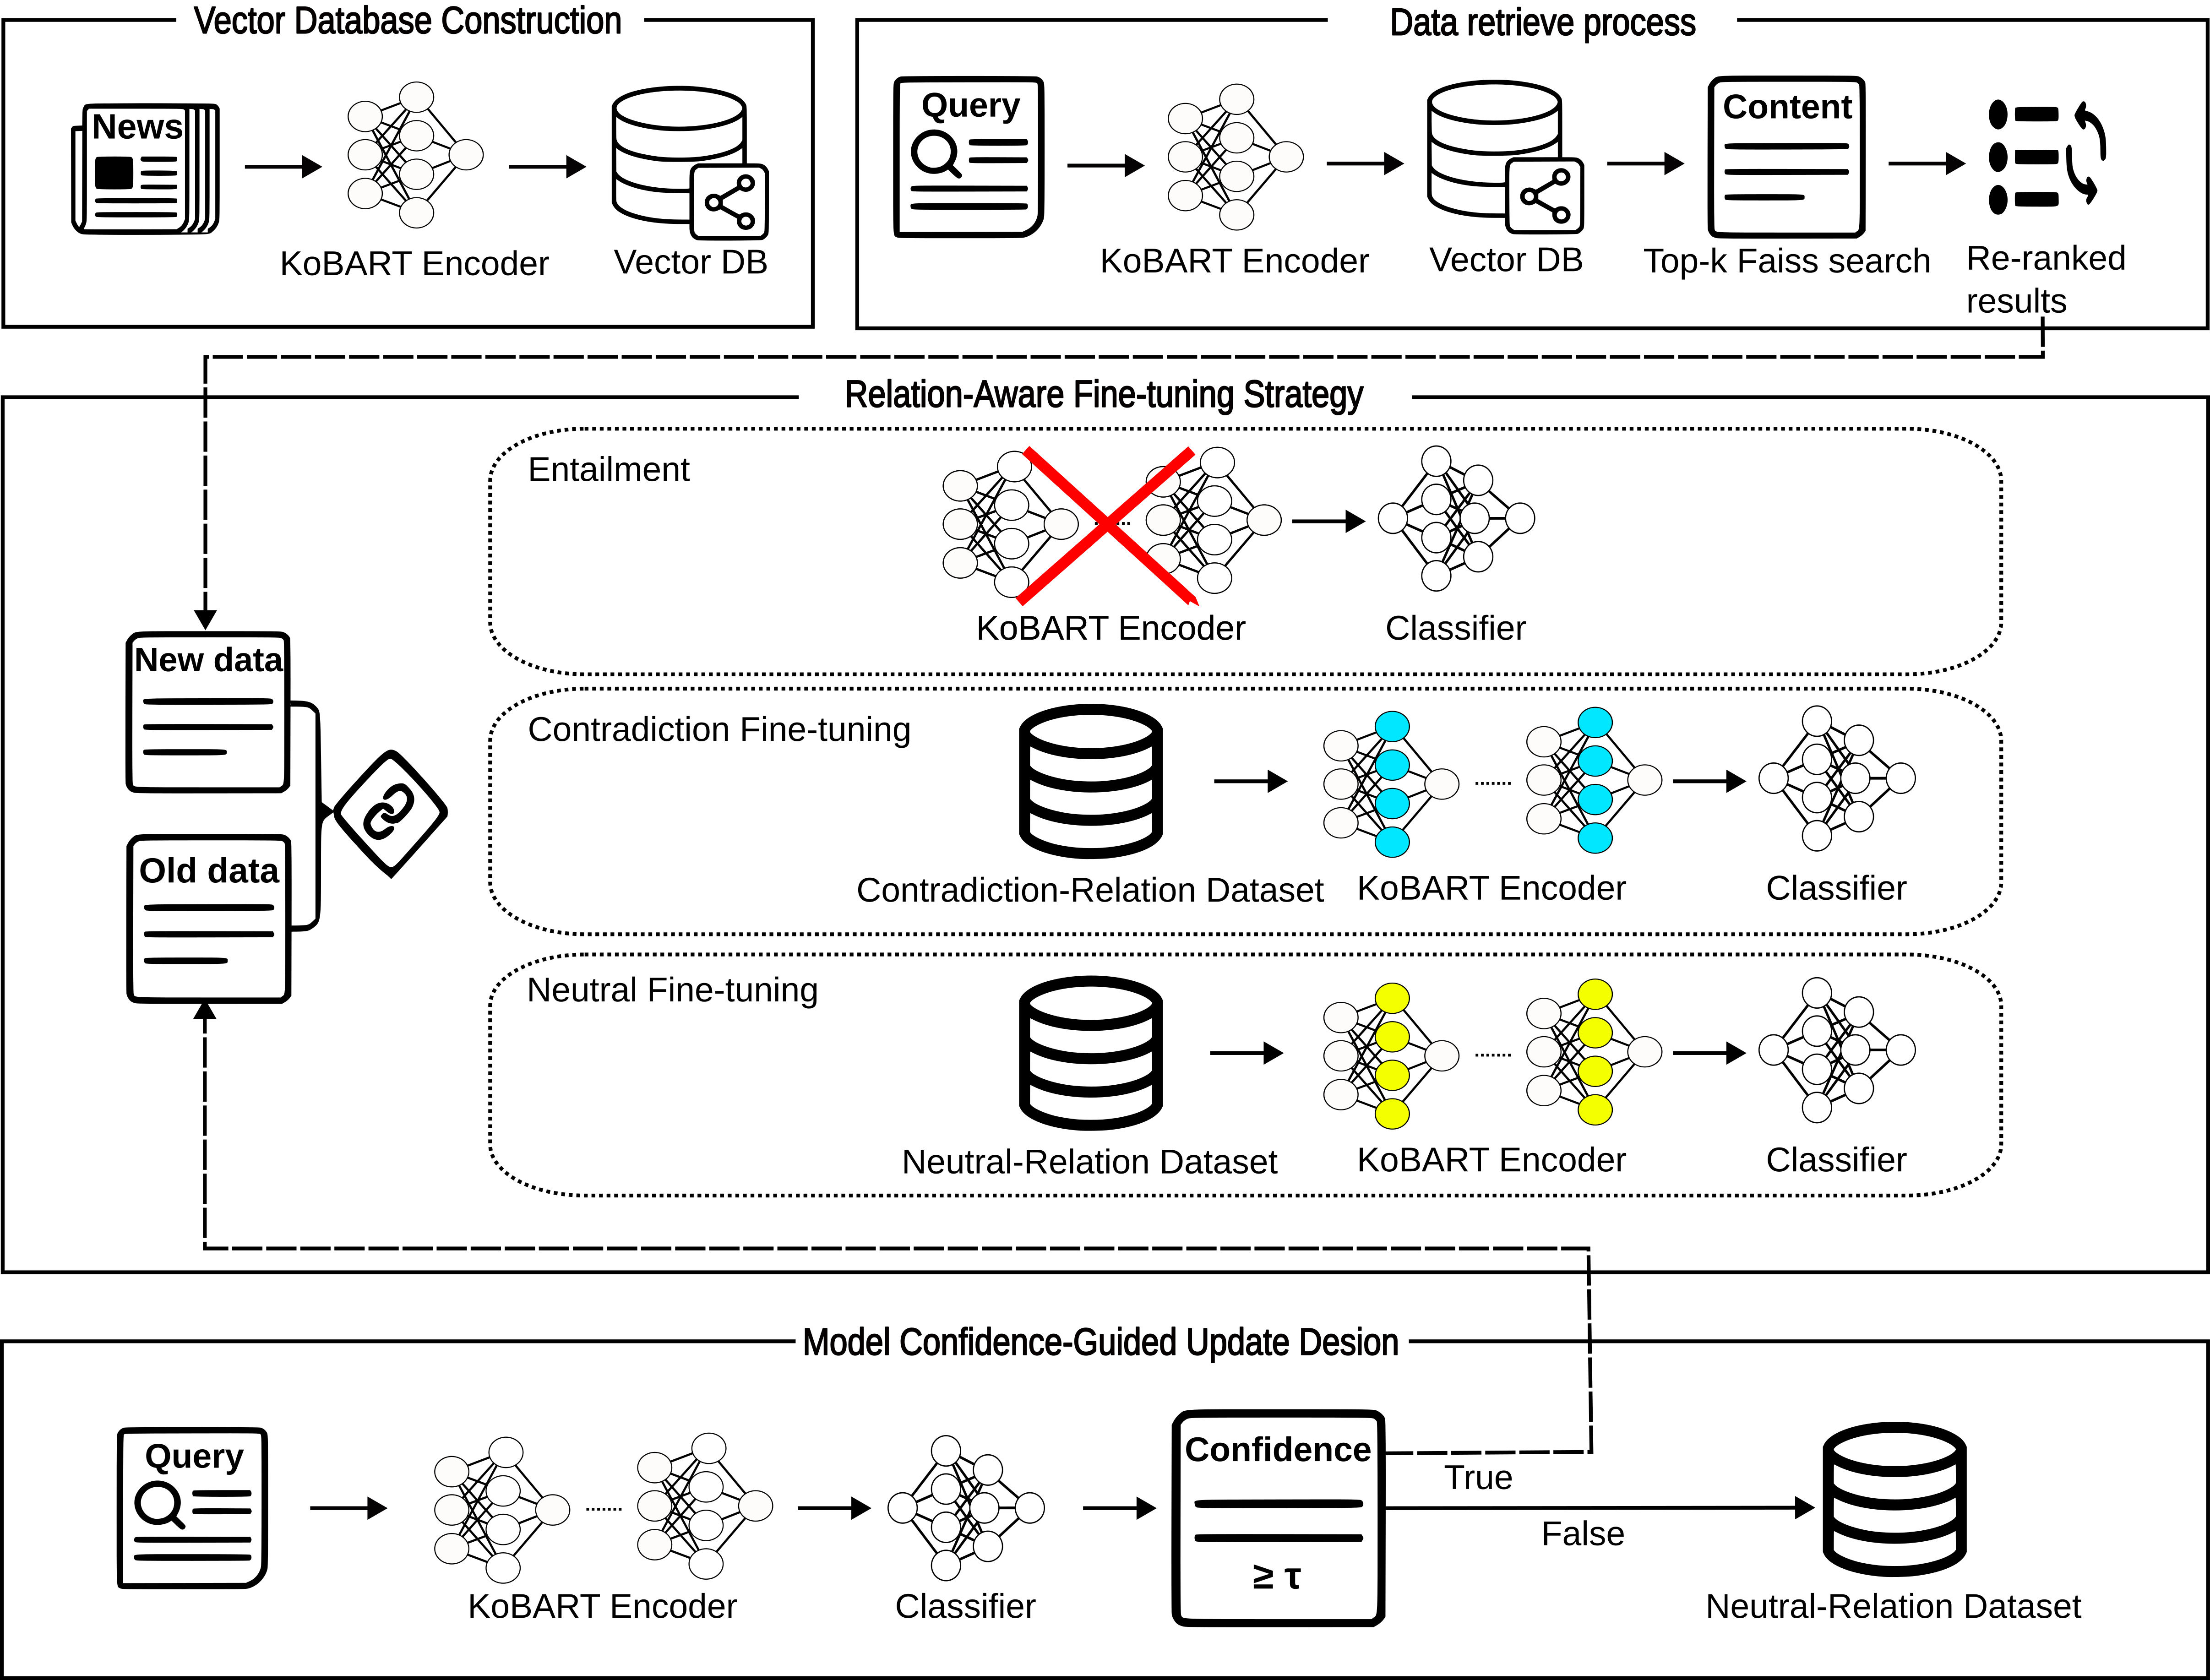
\includegraphics[width=\textwidth]{architecture.png}
    \caption{The architecture }
\end{figure}

그림 1은 Relation-aware Fine-tuning 프레임워크의 전반적인 동작 과정을 시각적으로 보여준다. 본 시스템은 의미적 유사성과 논리적 일관성에 기반하여 선택적인 모델 Fine-tuning을 수행하며, 크게 네 단계로 구성된다.
좌측 상단의 'Vector Database Construction' 단계에서는 KoBART 인코더를 활용해 새로운 뉴스 문장들을 임베딩하고, FAISS 기반 벡터 데이터베이스를 구축한다.

입력 문장은 KoBART 인코더를 통해 임베딩되고, FAISS를 통해 유사 문장이 검색되며, Cross-Encoder로 재랭킹된 후, NLI 관계 분석을 거쳐 selective fine-tuning 여부가 결정된다.

'Data Retrieve Process'는 새로운 질의 문장이 주어졌을 때 KoBART 인코더를 통해 임베딩된 후, 벡터 DB에서 의미적으로 유사한 문장들을 검색하고 Cross-Encoder를 통해 재정렬되는 과정을 나타낸다.

'Relation-Aware Fine-tuning Strategy' 블록은 검색된 문장과 기존 모델 출력 간의 논리적 관계(NLI: Entailment, Contradiction, Neutral)를 분류하는 단계를 표현하며, 선택적으로 fine-tuning이 수행된다.

'Model Confidence-Guided Update Design' 영역은 모델의 softmax 기반 model confidence score가 일정 임계값(τ ≥ 0.7)을 초과할 때에만 관계 분석과 fine-tuning이 수행됨을 의미하며, 과도한 업데이트를 방지하고 안정성을 높인다.

이와 같이 Figure 1은 Recognition → Association → Mastery로 이어지는 전체 시스템의 핵심 흐름을 효과적으로 요약하고 있으며, 기존 KME 접근과의 차별성과 실용적 구조를 강조한다. 
Relation-aware Fine-tuning은 단순한 fine-tuning을 넘어, Knowledge-Based Editing의 고도화된 형태로 볼 수 있으며, 다음과 같은 세 단계를 모두 만족한다:

\begin{itemize}
    \item{\textbf{Recognition Phase}:
    모델이 RAG(Retrieval-Augmented Generation) 구조에 기반하여 외부 벡터 데이터베이스로부터 새로운 정보를 인식한다.  
    이 단계에서는 KoBART 인코더를 활용해 질의 문장을 임베딩한 후, FAISS를 이용해 의미적으 로 유사한 문장을 검색한다.}
    
    \item{\textbf{Association Phase}:
    검색된 정보와 기존 모델 출력 간 관계를 분석한다. 이 과정에서 Cross-Encoder를 통해 재정렬된 검색 문장과 KoBART 모델의 출력 결과를 비교하여, NLI 기반 분류기를 통해 이들 간의 관계를 함의(Entailment), 모순(Contradiction), 중립(Neutral) 중 하나로 판별한다.}
    
    \item{\textbf{Mastery Phase}:
    
    관계 분석 결과에 따라, 해당 문장을 활용하여 선택적 fine-tuning을 수행한다. 이때 전체 모델이 아닌 특정 파라미터(인코더 MLP 레이어)만 업데이트됨으로써, 최소한의 수정으로 지식이 편집된다.
    }

\end{itemize}  

Knowledge-based editing 방식은 전통적으로 단일 문장 또는 단일 사실 삽입에 초점을 맞췄지만, 본 연구의 Relation-aware Fine-tuning은 지식의 관계성(relation)을 중심으로 업데이트 여부를 결정함으로써, 더 높은 정합성과 효율성을 확보한다. 




\subsection{KoBART-based Binary Classifier Design}

KoBART는 BART(Seq2Seq Transformer)의 한국어 특화 버전으로, 인코더-디코더 구조를 기반으로 한다. 
BART는 텍스트 복원 및 생성 태스크를 위해 설계되었으며, 인코더는 입력 문장을 Transformer로 인코딩하고, 디코더는 이를 바탕으로 시퀀스를 생성하는 구조를 가진다. 
해당 모델은 뉴스 기사, 위키피디아, 국립국어원의 모두의 말뭉치 등 다양한 한국어 코퍼스를 활용하여 Denoising Auto-Encoding 방식으로 사전 학습되었다. 
이러한 사전 학습을 통해 KoBART는 한국어 문장에 대한 풍부한 언어적 문맥을 학습하였으며, 본 연구에서는 이를 COVID-19 가짜 뉴스 탐지를 위한 이진 분류기로 전환하여 활용하였다.

입력 문장은 KoBART 인코더를 통해 인코딩되며, 인코더의 출력 중 평균 풀링된 임베딩이 의미 표현의 대표값으로 사용된다.
이후 해당 표현은 분류기(classification head)에 전달되어 softmax 함수를 통해 레이블 0(fakeness) 또는 1(realness)로 직접 분류된다. 

이와 같은 구조는 디코더를 사용한 생성 기반 응답 방식 대신, 간결하고 효율적인 이진 분류를 가능하게 하며, 모델의 출력 해석을 명확히 하고 학습 안정성을 높이는 데 기여한다. 
또한 KoBART의 사전학습된 언어적 지식은 한국어 문장에 대한 풍부한 문맥 이해를 가능하게 하며, downstream fine-tuning 시 높은 성능을 보장한다.

모델은 주어진 입력 문장 \( x \in \mathcal{D}_{\text{old}} \)에 대해, 해당 문장이 사실(True)인지 거짓(False)인지를 분류하기 위해 다음과 같은 절차를 따른다.
여기서 \( \mathbf{h}_i \)는 인코더의 \( i \)번째 토큰에 대한 은닉 상태이며, \( L \)은 전체 입력 토큰의 개수이다. 
\( W \)와 \( \mathbf{b} \)는 학습 가능한 분류기 파라미터를 의미한다. 
\begin{equation}
    \mathbf{x}_{\text{input}} = \text{Tokenizer}(x), \quad \text{where} \quad x \in \mathcal{D}_{\text{old}}, \; y \in \{0, 1\}
\end{equation}
\begin{equation}
    \text{hidden representation } \mathbf{h}  = \text{KoBART Encoder}(\mathbf{x}_{\text{input}}) 
\end{equation}
\begin{equation}
    \hat{\mathbf{y}} = \mathrm{softmax}\left( W \cdot \left( \frac{1}{L} \sum_{i=1}^{L} \mathbf{h}_i \right) + \mathbf{b} \right)
\end{equation}
\noindent

\begin{equation}
    \mathcal{L} = -\frac{1}{N} \sum_{i=1}^{N} \left[ y_i \log \hat{y}_i + (1 - y_i) \log (1 - \hat{y}_i) \right]
\end{equation}

여기서 \( \mathrm{conf}(x) \)는 softmax 출력 확률 중 최대값을 의미하며, 이는 모델이 입력 \( x \)에 대해 얼마나 높은 신뢰도를 갖고 있는지를 나타낸다. 
또한, 모델의 예측 레이블 \( y_{\text{old}} \)는 다음과 같이 정의되며, 이후 NLI 기반 관계 판단 및 selective fine-tuning 과정에서 기준값으로 활용된다.
분류 결과로부터 얻은 예측 확률 분포 \( \hat{\mathbf{y}} \)를 기반으로, 모델의 해당 입력에 대한 신뢰도(confidence)는 다음과 같이 정의된다:
\begin{equation}
    \mathrm{conf}(x) = \max \left( \hat{y}_0, \hat{y}_1 \right)
\end{equation}
\begin{equation}
    y_{\text{old}} = \arg\max_{k \in \{0, 1\}} \hat{y}_k
\end{equation}



\subsection{External Knowledge Retrieval and Semantic Re-ranking}

Relation-aware Fine-Tuning에서 핵심적인 역할을 수행하는 또 다른 구성 요소는 외부 지식 검색 모듈이다. 
이 모듈은 KoBART 인코더를 활용하여 입력 문장을 고차원 임베딩으로 변환한 후, FAISS(Facebook AI Similarity Search) 기반의 벡터 데이터베이스를 구성하고, 의미적으로 유사한 문장을 검색하는 데 활용된다. 
이 전체 과정은 크게 두 단계로 구성된다.
\begin{itemize}
    \item{\text{Vector Database Construction and Top-k Query Retrieval using FAISS}}
    \item{\text{Cross-Encoder Re-ranking}}
\end{itemize}  

\subsubsection{Vector Database Construction and Top-k Query Retrieval using FAISS}


KoBART 인코더의 마지막 히든 상태들을 평균 풀링하여 각 문장의 고차원 임베딩 벡터 \( \mathbf{v}_{x'} \)를 생성하고, 이를 FAISS 인덱스 \( \mathcal{I} \)에 삽입한다. 
여기서 \( x' \in \mathcal{D}_{\text{new}} \)는 새로운 데이터 샘플을 의미하며, \( \mathbf{v}_{x'} \)는 해당 샘플로부터 생성된 임베딩 벡터이다. 
\( L \)은 입력 문장의 토큰 개수를 나타내고, \( \mathcal{I} \)는 FAISS 기반으로 구성된 벡터 인덱스이다. 
연산 \( \mathcal{I} \cup \{ \cdot \} \)는 새로운 임베딩을 벡터 데이터베이스에 추가하는 과정을 나타낸다. 

\begin{equation}
    \mathbf{v}_{x'} = \frac{1}{L} \sum_{i=1}^{L} \mathrm{Encoder}(\mathrm{Tokenizer}(x'_i)), \quad \text{where} \quad x' \in \mathcal{D}_{\text{new}}, \; y' \in \{0, 1\}
\end{equation}

\begin{equation}
    \mathcal{I} \leftarrow \mathcal{I} \cup \left\{ \mathbf{v}_{x'} \;\middle|\; x' \in \mathcal{D}_{\text{new}} \right\}
\end{equation}


FAISS는 고차원 벡터 간 유사도 기반 검색을 빠르고 효율적으로 수행하기 위해 설계된 라이브러리로, L2 거리, 내적(dot product), 코사인 유사도 기반의 근사 최근접 이웃(Approximate Nearest Neighbor, ANN) 검색을 지원한다. 
다양한 인덱싱 구조를 제공하며, 정확도와 속도 간의 요구에 따라 선택적으로 조정할 수 있는 유연성을 갖춘다.
FAISS는 코사인 유사도 기반 검색을 직접 지원하지 않지만, 벡터 정규화를 통해 L2 거리 기반 검색과 동일한 효과를 얻을 수 있다. 

본 연구에서는 KoBART 인코더의 출력 임베딩을 단위 벡터로 정규화한 후, L2 거리 기반 인덱스를 적용하여 코사인 유사도와 동일한 검색 결과를 구현한다. 
이러한 설정은 문장 간 의미적 유사성을 효율적이면서도 정확하게 비교할 수 있게 한다.

사용자 질의 \( q \)는 동일한 방식으로 임베딩되어 벡터 표현 \( \mathbf{v}_q \)를 생성하며, FAISS 인덱스 \( \mathcal{I} \)에서 Top-\(k\)개의 유사 문장을 검색한다.
\( \mathrm{Retrieve}_k(q) \)는 질의 벡터 \( \mathbf{v}_q \)와 가장 유사한 \( k \)개의 벡터를 FAISS 인덱스에서 검색하는 연산을 나타내며, 유사도 계산은 벡터 간의 L2 거리 제곱 \( \ell_2^2 \)를 기반으로 수행되며,  \( \left\| \mathbf{v}_q - \mathbf{v}_{x'} \right\|_2^2 \)와 같이 정의된다.  
벡터 정규화를 선행할 경우, 이러한 L2 거리 기반 유사도 계산은 코사인 유사도 기반 검색과 동일한 효과를 제공한다.

\begin{equation}
    \mathbf{v}_q = \frac{1}{L} \sum_{i=1}^{L} \mathrm{Encoder}(\mathrm{Tokenizer}(q))_i
\end{equation}

\begin{equation}
    \mathrm{Retrieve}_k(q) = \arg\min_{\mathbf{v}_{x'} \in \mathcal{I}} \left\| \mathbf{v}_q - \mathbf{v}_{x'} \right\|_2^2
\end{equation}

\subsubsection{NLI-based Knowledge Editing Strategy}
FAISS로 검색된 후보 문장은 코사인 거리 기반의 단순 유사도만 반영되므로 문맥 일치 수준이 충분히 보장되지 않는다. 
이를 보완하기 위해 Cross-Encoder를 도입하여 쿼리 문장과 검색된 문장 쌍을 입력으로 하고, 보다 정밀한 의미 유사도 점수를 계산한다. 
이 점수를 기반으로 문장들을 재정렬하며, 최종적으로 가장 관련성 높은 문장이 상위에 위치하게 된다. 재랭킹된 결과는 이후 NLI 기반 관계 평가 및 selective fine-tuning에 활용된다.
이러한 이중 구조의 검색 시스템은 단순 벡터 유사도 기반 검색보다 정밀한 문장 선택이 가능하며, 새로운 정보와 기존 예측 간의 관계 판단에 더욱 신뢰성 있는 근거를 제공한다. 
또한, Cross-Encoder는 기존 COVID-19 데이터셋으로 fine-tuning된 모델로, 벡터 기반 similarity search보다 정밀한 문장 레벨의 의미 비교가 가능하여, 더 신뢰도 높은 문장을 선택할 수 있도록 한다. 

$f_{\text{encoder}}^{\text{cross}}(q, x')$는 Cross-Encoder 모델을 의미하며, 쿼리 $q$와 후보 문장 $x'$를 함께 입력하여 두 문장 간의 의미적 유사도를 계산한다.
$S_i$는 쿼리 $q$와 후보 문장 $x'_i$ 간의 의미 유사도로, Cross-Encoder $f_{\text{encoder}}^{\text{cross}}$를 통해 계산된다. 
이 중 $S_i$가 임계값 $\theta$를 초과하는 후보들 중에서 가장 높은 유사도를 갖는 문장의 레이블 $y_j$를 새로운 레이블 $y_{\text{new}}$로 정의한다.

\begin{equation}
    S_{\text{i}} = \mathrm{sim}(q, x'_i) = f_{\text{encoder}}^{\text{cross}}(q, x'_i)
\end{equation}

\begin{equation}
    y_{\text{new}} = y'_{j} \quad \text{where} \quad j = \arg\max_{S_i > \theta} S_i
\end{equation}
    


\subsection{Related-Aware Fine-tuning}

기존 출력(Old data)과 검색된 새로운 정보(New data) 간의 논리적 관계를 분석하고, 그 관계 유형에 따라 모델 업데이트 여부 및 방식을 selective하게 결정하는 Relation-aware Fine-tuning 전략을 제안한다. 
이 전략은 모델의 불필요한 파라미터 변경을 최소화하면서, 최신 정보 반영과 기존 지식 유지 간의 균형을 동시에 달성하는 데 목적이 있다.
본 연구는 이러한 NLI 구조를 모델 지식 편집(Knowledge Editing)이라는 새로운 문제 영역에 적용하여, 기존 Knowledge-based Model Editing(KME) 기법들과 구별되는 새로운 패러다임을 제안한다.
본 절에서는 KoBART 모델의 응답 결과(Old data)와 외부 벡터 데이터베이스로부터 검색된 문장(New data) 간의 의미적 관계를 판단하고, 그 결과를 바탕으로 모델 파인튜닝 전략을 결정하는 전체 과정을 기술한다. 

이 관계 판단은 Bowman et al. (2015)이 제안한 자연어 추론(Natural Language Inference, NLI) 프레임워크에 기반한다. 
해당 프레임워크는 전제(premise)와 가설(hypothesis) 간의 의미 관계를 함의(Entailment), 모순(Contradiction), 중립(Neutral)의 세 가지로 분류하며, 텍스트 간 논리적 일관성과 추론 기반 연관성을 정밀하게 분석할 수 있다는 점에서 일반성을 제공한다.
본 연구에서는 모델의 기존 출력(Old data)을 NLI 구조상의 premise로, 외부 검색을 통해 얻은 새로운 문장(New data)을 hypothesis로 간주한다. 
전제는 모델이 내재적으로 보유한 지식에 기반해 생성한 응답이고, 가설은 외부 지식원으로부터 획득한 최신 정보이다.

이 두 문장 간 관계가 Entailment일 경우 모델 업데이트는 필요하지 않으며, Contradiction일 경우 기존 지식을 새로운 정보로 대체하고, Neutral일 경우 두 문장을 함께 고려하여 파인튜닝을 수행한다.

이와 같은 관계 분석은 단순히 새로운 정보를 삽입하는 기존 KME 접근들과 본 연구를 명확히 구분짓는다. 
기존 ROME, MEMIT 등은 지식 insertion에 초점을 맞추어, 기존 지식과의 충돌 여부를 사전에 평가하지 않고, 삽입 후 catastrophic forgetting, inconsistency과 같은 부작용에 대해서도 별다른 대응책을 마련하지 못했다.
반면, 본 연구의 Relation-aware Fine-tuning은 삽입(insert) 이전에, 기존 지식과 새로운 정보 간의 논리적 관계를 사전 평가하고, 이 평가 결과에 따라 업데이트 여부와 방식을 다르게 결정한다는 점에서 근본적으로 다르다. 
이를 통해 불필요한 파라미터 변경을 줄이는 한편, 모델의 일관성(Locality)과 최신성(Generality) 확보를 동시에 달성할 수 있다.

관계 유형은 다음과 같으며, 각 경우에 따라 fine-tuning 전략이 달라진다:

\begin{itemize}
    \item{\textbf{Entailment}:
    Old data가 New data를 논리적으로 포함하는 경우이다. 즉, 모델의 기존 응답이 최신 정보와 일관될 때를 의미하며, 이 경우 모델은 이미 해당 정보를 내재화하고 있으므로, 추가적인 업데이트를 수행할 필요가 없다.}
    \item{\textbf{Contradiction}:
    Old data와 New data가 명확히 모순되는 경우이다. 이는 기존 응답이 최신 정보와 충돌하는 상황으로, 모델의 내부 지식이 잘못되었을 가능성이 높다고 판단된다. 
    따라서, 기존 파라미터를 삭제하고 새로운 정보를 반영하는 fine-tuning이 필요하다.}
    \item{\textbf{Neutral}:
    Old data와 New data 간에 명확한 포함 관계나 모순 관계가 성립하지 않는 경우이다. 이때 새로운 정보는 기존 지식에 대해 독립적이거나 보완적인 성격을 지니며, 새로운 정보를 함께 반영하는 방향으로 fine-tuning을 진행한다.
    }
\end{itemize}  
이러한 관계 유형은 모델의 기존 응답(Old data)과 검색된 정보(New data) 간의 의미적 대응을 기반으로 정의된다.  
특히 관계 판단은 모델이 해당 쿼리 \( q \)에 대해 충분히 높은 신뢰도(confidence)를 보일 때에만 유효하게 수행된다.

쿼리 \( q \)에 대해, 사전 학습된 모델이 출력한 예측 결과를 \( y_{\text{old}} \), 벡터 데이터베이스에서 검색된 문장 \( x' \)의 레이블을 \( y_{\text{new}} \)라고 정의한다.  
여기서 \( \mathrm{conf}(q) \)는 쿼리 \( q \)에 대한 softmax 출력 중 최대 확률값을 의미하며, \( \tau \)는 사전에 설정된 confidence 임계값(threshold)이다.  

관계 판단은 모델의 예측 확신도와 검색된 정보 간의 레이블 일치 여부를 함께 고려하여 이루어진다.  
두 문장 \( x \)와 \( x' \) 간의 논리 관계 \( r(x, x') \)는 다음과 같이 정의된다:

\begin{equation}
    r(x, x') =
    \begin{cases}
    \text{entailment}, & \text{if } y_{\text{old}} = y_{\text{new}} \;\land\; \mathrm{conf}(q) > \tau \\
    \text{contradiction}, & \text{if } y_{\text{old}} \ne y_{\text{new}} \;\land\; \mathrm{conf}(q) > \tau  \\
    \text{neutral}, & \text{otherwise}
    \end{cases}
    \end{equation}


\subsection{Relation-Aware Fine-Tuning}
   
 본 연구에서는 관계 분류 결과를 기반으로 selective fine-tuning 뿐만 아니라, 학습 손실 함수(loss function) 설계에도 반영하여, Contradiction 경우에는 적극적인 파라미터 수정, Neutral 경우에는 보완적 학습, Entailment 경우에는 학습 스킵 전략을 적용한다. 
 이러한 일관된 설계는 모델 업데이트 과정 전반에 걸쳐 논리적 근거에 기반한 결정이 이루어지도록 보장한다.

전체 flow를 보여준다.
\begin{figure}[htbp]
    \centering
    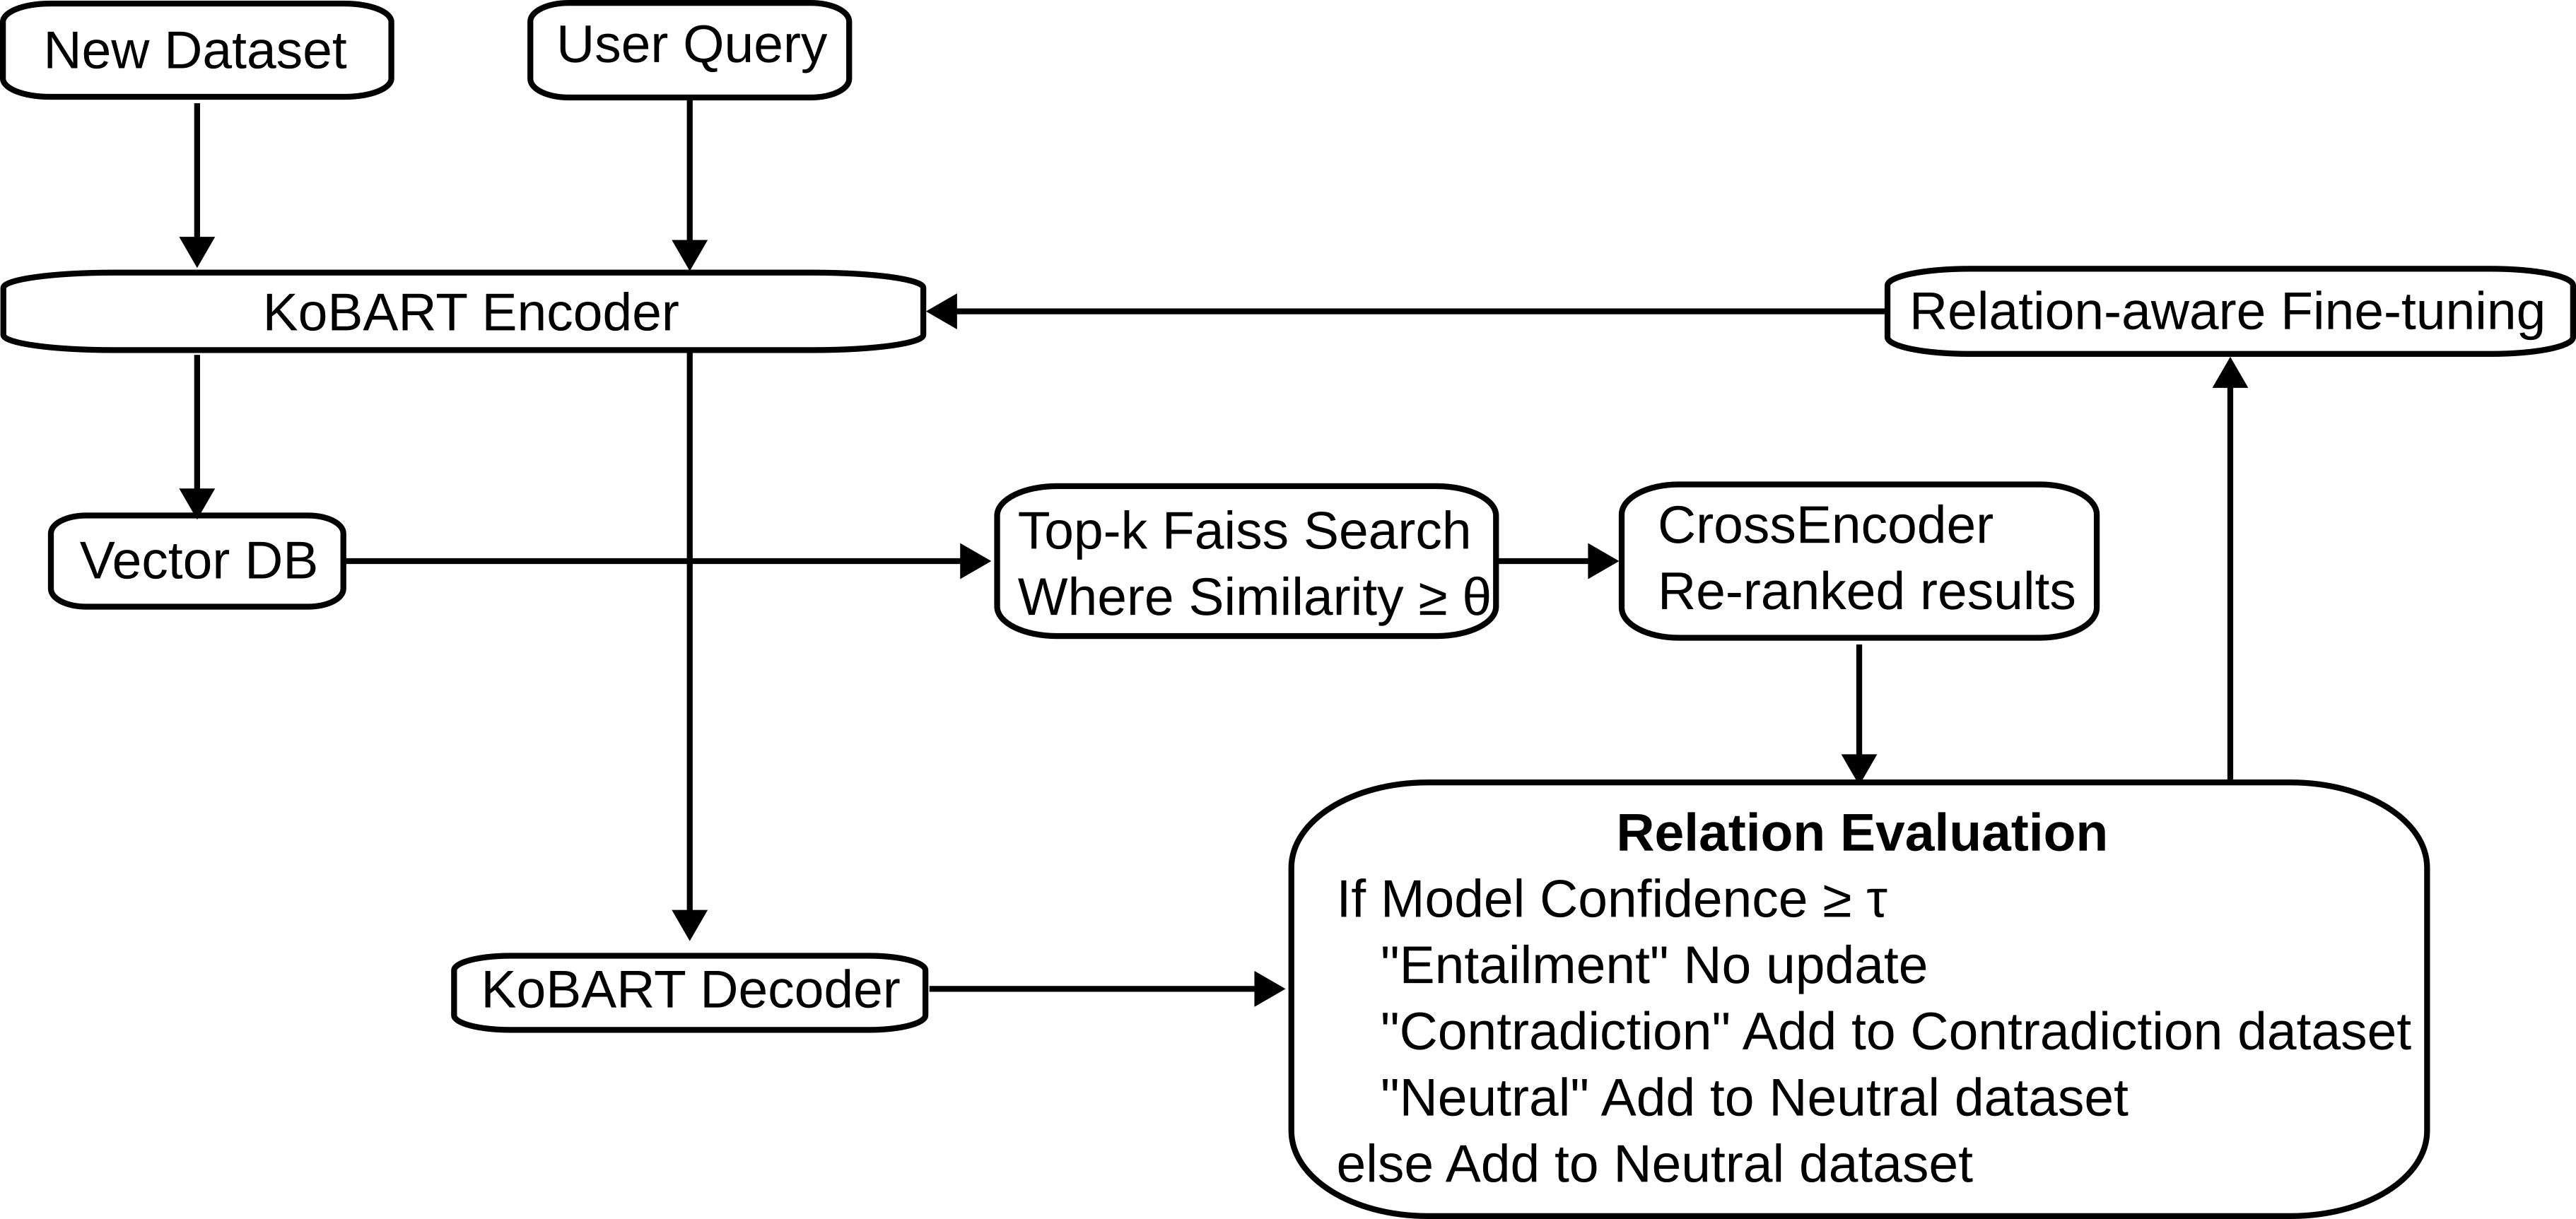
\includegraphics[width=\textwidth]{flow.png}
    \caption{The architecture }
\end{figure}


여기서 관계에 따른 loss function설명
이 관계 분류에 따라 다음과 같은 fine-tuning 전략이 적용된다:
특히 Contradiction 관계가 감지된 경우, 단순한 fine-tuning이 아니라 다음과 같은 특수한 손실 함수(loss function)를 적용하여 모델 파라미터를 업데이트한다. 모델의 출력 로짓을 z, 정답 레이블을 y라 할 때, 반대 레이블은 1−y로 정의된다. 이때 Contradiction 상황에서의 총 손실은 다음과 같이 계산된다:

    

\begin{equation}
    \mathcal{L}_{\text{contradiction}} =
    \underbrace{y_{\text{new}} \log \hat{y}_1 + (1 - y_{\text{new}}) \log \hat{y}_0 }_{\mathcal{L}_{\text{true}}}
    -\, \alpha \cdot
    \underbrace{ y_{\text{old}} \log \hat{y}_1 + (1 - y_{\text{old}}) \log \hat{y}_0 }_{\mathcal{L}_{\text{false}}}
\end{equation}

        
여기서:

    CE(z,y)는 로짓 z와 정답 레이블 y를 사용한 Cross-Entropy 손실,

    αα는 조정 계수로, 본 연구에서는 α=0.1로 설정하였다.

이는 모델이 정답(label y)에 대해 손실을 줄이는 동시에, 이전 예측(label 1−y)에 대해 손실을 늘리는 방향으로 학습되도록 유도한다. 이를 통해 모델은 기존 잘못된 지식을 능동적으로 수정할 수 있다.

반면 Neutral 관계가 감지된 경우에는 일반적인 fine-tuning 방식과 동일하게, 정답 레이블 y에 대해 단순 Cross-Entropy 손실을 최소화한다:

\begin{equation}
    \mathcal{L}_{\text{neutral}} = {y_{\text{new}} \log \hat{y}_1 + (1 - y_{\text{new}}) \log \hat{y}_0}
\end{equation}

이러한 관계 기반 손실 함수 설계는 모델이 논리적 모순에 민감하게 반응하고, 필요할 때만 선택적으로 업데이트를 수행하며, 모델의 일관성과 최신성을 동시에 확보할 수 있도록 한다.
결론적으로, 본 연구는 NLI 프레임워크를 Knowledge Editing 문제에 창의적으로 적용하여, 기존 KME 기법 대비 한층 정교하고 일관성 있는 모델 지식 업데이트 방법론을 제안하며, 이는 본 논문의 가장 중요한 기여 중 하나이다.


pseudocode


생성된 응답과 검색된 문서 간 관계 판단 기준

본 시스템에서의 NLI 기반 관계 분류는 단독 기법이 아니라 Knowledge-based Editing을 확장한 형태로 이해할 수 있다. 특히 기존 KME 방식에서는 주로 Mastery Phase(내부 파라미터 수정)에만 초점을 맞췄던 반면, 본 연구는 Recognition → Association → Mastery의 세 단계를 구조화하여 다음과 같이 설계하였다:

Recognition Phase: 외부 벡터 데이터베이스에서 FAISS + KoBART 인코더를 통해 문장을 검색하는 과정으로, 이는 RAG의 retrieval 방식에 해당한다.

Association Phase: Cross-Encoder와 cosine similarity를 통해 검색된 문장과 기존 출력 간 관계를 정의한다.

Mastery Phase: 판단된 관계에 따라 selective fine-tuning을 수행하는 단계로, Contradiction일 경우만 파라미터를 업데이트한다.


%============================================================%
% Experiments
%============================================================%


\section{Experiments}

\subsection{Dataset Configuration}

본 연구에서는 COVID-19 가짜 뉴스 탐지를 위한 다양한 시기의 데이터셋을 활용하여 제안한 모델의 지식 유지 및 갱신 능력을 평가하였다.
특히, 시간적 도메인 분리 전략을 통해 모델이 새로운 정보에 노출되었을 때 어떻게 반응하고, 기존 지식과의 관계를 어떻게 조정하는지를 시뮬레이션하였다.
전체 데이터는 수집 시점에 따라 두 가지 도메인으로 구분된다.  
2019년에 수집된 영어 기반 데이터는 \textbf{Old data}로 정의되며, 모델의 초기 지식 기반(pretraining corpus)으로 사용된다.  
반면, 2021년 이후 수집된 최신 한국어 기반 데이터는 \textbf{New data}로 정의되며, 모델이 이후에 검색 또는 fine-tuning을 통해 참조하는 외부 정보로 활용된다.

2019년에 수집된 영어 기반 데이터는 "Old data"로, 2021년에 수집된 한국어 기반 데이터는 "New data"로 정의된다. 
이를 통해, 실제 환경에서 새로운 정보가 유입되었을 때 모델이 어떻게 갱신될 수 있는지를 시뮬레이션하고자 하였다.

\begin{itemize}
    \item{\textbf{Old Data}:
    Old data는 2019년 Kaggle에서 공개된 영어 기반의 COVID-19 가짜 뉴스 데이터셋을 기반으로 하며, 당시는 한국어로 구성된 고품질의 관련 데이터셋이 부재하였다.  
    이에 따라 본 연구에서는 해당 영어 문장을 Google Translator를 활용하여 한국어로 자동 번역하였고, 이 결과물을 한국어 기반의 사전 학습 코퍼스로 활용하였다.  
    생성된 데이터는 언어적 자연스러움이 다소 떨어질 수 있으나, 초기 지식 기반 구축 및 도메인 적응 전 모델 성능 측정을 위한 비교 기준 데이터로 적절하다.}
    \item{\textbf{New Data}:
    New data는 실제 한국어 환경에서 모델의 지식 갱신 상황을 비교실험하기 위해 설계되었다.  
    서울대학교 FactCheck, 백신 팩트체크 프로젝트, 질병관리청(KDCA) 공식 홈페이지 등 다양한 국내 팩트체크 플랫폼으로부터 COVID-19 관련 문장을 수집하였다.  
    수집된 데이터는 Lee and Kim (2022)에서 제시한 프로토콜에 따라 정제 및 라벨링되었으며, 총 3,500개의 문장(진짜: 1,500건, 가짜: 1,500건)으로 구성된다.  
    해당 데이터는 모델 평가뿐 아니라, 벡터 DB 구축 및 NLI 기반 fine-tuning에 활용되는 핵심 자료로 기능한다.}
    
\end{itemize}  
두 데이터셋 모두 모델 학습과 평가의 일관성을 유지하기 위해 동일한 전처리 과정을 거쳤다:

\begin{itemize}
    \item{\textbf{Label Mapping}:
    데이터 내 다양한 레이블 표현을 이진 분류 기준(True = 1, False = 0)으로 통일하였다.}
    \item{\textbf{Text Filtering}:
    기사 제목, 출처, 발화자 등 부수적인 메타 정보를 제거하고, 본문 문장만을 추출하였다.  
    이는 문장 수준의 판단에 집중하기 위한 전처리 단계이다.}
    \item{\textbf{Tokenization}: 
    모든 문장은 KoBART 토크나이저를 사용하여 서브워드 단위로 토큰화되었으며, 모델 입력의 길이를 통일하기 위해 padding 및 truncation을 수행하였다.
    }
\end{itemize}  

이와 같은 일관된 전처리 전략은 서로 다른 시점과 출처를 가진 데이터셋 간의 정량적 비교를 가능하게 하며, 문장 단위의 신뢰도 평가를 위한 기초 작업으로 기능한다.  
최종적으로 Old data는 모델의 사전 학습(pretraining) 단계에서 사용되고, New data는 추론 시점에서 검색 및 fine-tuning을 위한 외부 데이터로 활용된다.

configuration

\subsection{Evaluation Metrics}

본 연구에서는 Relation-aware Fine-tuning의 효과를 다각도로 분석하기 위해 세 가지 주요 평가 지표를 사용하였다: Accuracy, Locality, Generality.


Accuracy는가장 기본적인 성능 지표로서, 모델이 입력 문장에 대해 올바른 진실성 판단(True or False)을 내렸는지 여부를 측정한다.  
사용된 COVID-19 가짜 뉴스 데이터셋은 클래스 간 분포가 균등하게 구성되어 있어, 불균형 보정이 필요 없으며 Accuracy 지표가 대표성을 가진다.  
Accuracy는 전체 샘플 수 \( N \)에 대해 모델의 예측값 \( \hat{y}_i \)가 실제 정답 \( y_i \)와 일치하는 비율로 정의되며, 다음과 같이 수식으로 표현된다:
\begin{equation}
    \text{Accuracy} = \frac{\text{Number of Correct Predictions}}{\text{Total Number of Samples}}
\end{equation}

Locality는 모델이 특정 지식을 편집한 이후에도, 편집과 무관한 입력에 대해 기존 동작을 얼마나 유지하는지를 측정하는 지표이다.
이는 모델 편집의 국소성(localized effect)을 평가하며, 기존 지식에 대한 불필요한 간섭(catastrophic forgetting)을 방지하는 데 핵심적인 역할을 한다.
본 연구에서는 Relation-aware Fine-tuning이 편집 대상 외 지식에 미치는 영향을 최소화하는지를 평가하기 위해, 다음과 같은 방식으로 Locality를 정의한다.
여기서 \( \mathcal{X}_{\text{unedit}} \)는 편집 대상과 무관한 입력 집합이며, \( f \)는 편집 전 모델, \( f^* \)는 편집 후 모델을 나타낸다.

\begin{equation}
\text{Locality} = \frac{1}{\left| \mathcal{X}_{\text{unedit}} \right|} \sum_{x \in \mathcal{X}_{\text{unedit}}} \mathbb{1} \left[ f(x) = f^*(x) \right]
\end{equation}



 
Generality는 편집된 지식이 새로운 상황이나 표현에도 일반화되어 적용되는지를 평가하는 지표이다.  
즉, 단일 문장 또는 사실(fact)에 대한 지식 편집이, 그와 의미적으로 유사한 다른 문장들에도 일관되게 반영되는지를 측정한다.  
이는 단순한 정합성(consistency)을 넘어, 모델의 추론 능력과 지식 확장 가능성을 나타낸다.
본 연구에서는 편집 후 모델을 \( f^* \), 편집 목표 출력을 \( y^* \), 편집된 지식과 의미적으로 유사한 테스트 입력 집합을 \( \mathcal{X}_{\text{gen}} \)이라 정의하며, Generality는 다음과 같이 수식으로 표현된다.

\begin{equation}
\text{Generality} = \frac{1}{\left| \mathcal{X}_{\text{gen}} \right|} \sum_{x \in \mathcal{X}_{\text{gen}}} \mathbb{1} \left[ f^*(x) = y^* \right]
\end{equation}


특히 ROME, MEMIT 등 기존 Knowledge Editing 연구에서는 모델 편집의 안정성과 선택성(selectivity)을 정량적으로 평가하기 위해 Locality와 Generality를 모두 핵심 지표로 활용해 왔다.
이들 연구는 단일 사실을 편집한 이후에도, 그와 관련된 다양한 문장 및 문맥에서 일관된 예측을 유지하는 능력이 모델 편집의 실질적 효과를 판단하는 중요한 기준임을 강조하였다.

이러한 평가지표는 단순한 예측 정확도만으로는 확인할 수 없는 편집의 품질을 평가하는 데 필수적이다.  
특히 KME 연구에서는 Locality와 Generality를 모두 충족하는 것이 이상적이나, 많은 기존 기법들은 이 두 속성 간 균형을 유지하는 데 어려움을 겪고 있다.  
본 연구는 NLI 기반 평가를 통해 관계 중심의 selective editing을 수행함으로써, Locality와 Generality를 동시에 향상시키는 것을 목표로 한다.



\subsection{Ablation Studies}

\subsubsection{Comparison of decoder-inclusive and encoder-only architectures}

본 실험에서는 KoBART의 디코더를 포함한 구조(Encoder + Decoder + Classifier)와, 디코더를 제거하고 인코더 출력에 직접 분류기를 연결한 구조(Encoder + Classifier)를 비교하여, 분류 안정성과 학습 효율성을 분석하였다.

두 구조 모두 동일한 학습 조건과 데이터셋을 기반으로 학습되었으며, 네 가지 손실 지표 true loss, false loss, neutral loss, total loss를 중심으로 비교 분석하였다.  

그림 3은 각 loss 항목의 변화 추이를 시각화한 결과이다.  
본 연구에서 정의한 손실 함수 \( \mathcal{L}_{\text{contradiction}} \)는 곧 total\_loss로, 그 구조적 특성상 학습이 진행될수록 모델은 기존 파라미터를 제거하는 방향으로 최적화되어야 한다.  
따라서 true loss는 점차 감소하고, false loss는 증가하는 경향을 보이는 것이 바람직하다.

이러한 조건에서 비교한 결과, Encoder-only 구조는 false loss를 제외한 true loss, neutral loss, total loss에서 더 낮은 값을 안정적으로 유지하였으며, 학습 초기부터 더 빠른 수렴 속도를 보였다. 
false loss에서는 Encoder-only 모델이 더 높은 값을 유지하여, 기존 잘못된 지식의 제거 측면에서도 효과적인 학습을 수행함을 확인할 수 있었다.

Decoder 포함 구조는 학습 초기에 진동(oscillation)이 두드러지며, 후반에는 수렴 안정성이 떨어지는 양상이 나타났다. 
이는 생성 기반 분류 방식이 디코더를 통한 문장 생성을 요구함에 따라, 파라미터 수 증가 및 학습 불안정성이 발생할 가능성을 시사한다.

결과적으로, Encoder-only 구조는 입력 문장의 각 토큰에 대한 hidden state의 평균 풀링을 통해 문장 임베딩을 생성함으로써, 학습 안정성과 파라미터 효율성 측면 모두에서 우수한 성능을 보였다.  
특히, neutral loss 및 total loss항목에서 보다 안정적인 하강 곡선과 빠른 수렴 속도를 나타내며, 생성 기반 구조보다 높은 분류 안정성을 확보하였다.  
이는 이진 분류와 같은 태스크에서, 디코더를 활용한 문장 생성 기반 접근법보다 단순하고 직접적인 인코더 기반 분류 방식이 더욱 실용적이고 효율적일 수 있음을 시사한다.

\begin{figure}[htbp]
    \centering
    
    % 첫 번째 줄
    \begin{subfigure}[b]{0.4\textwidth}
        \centering
        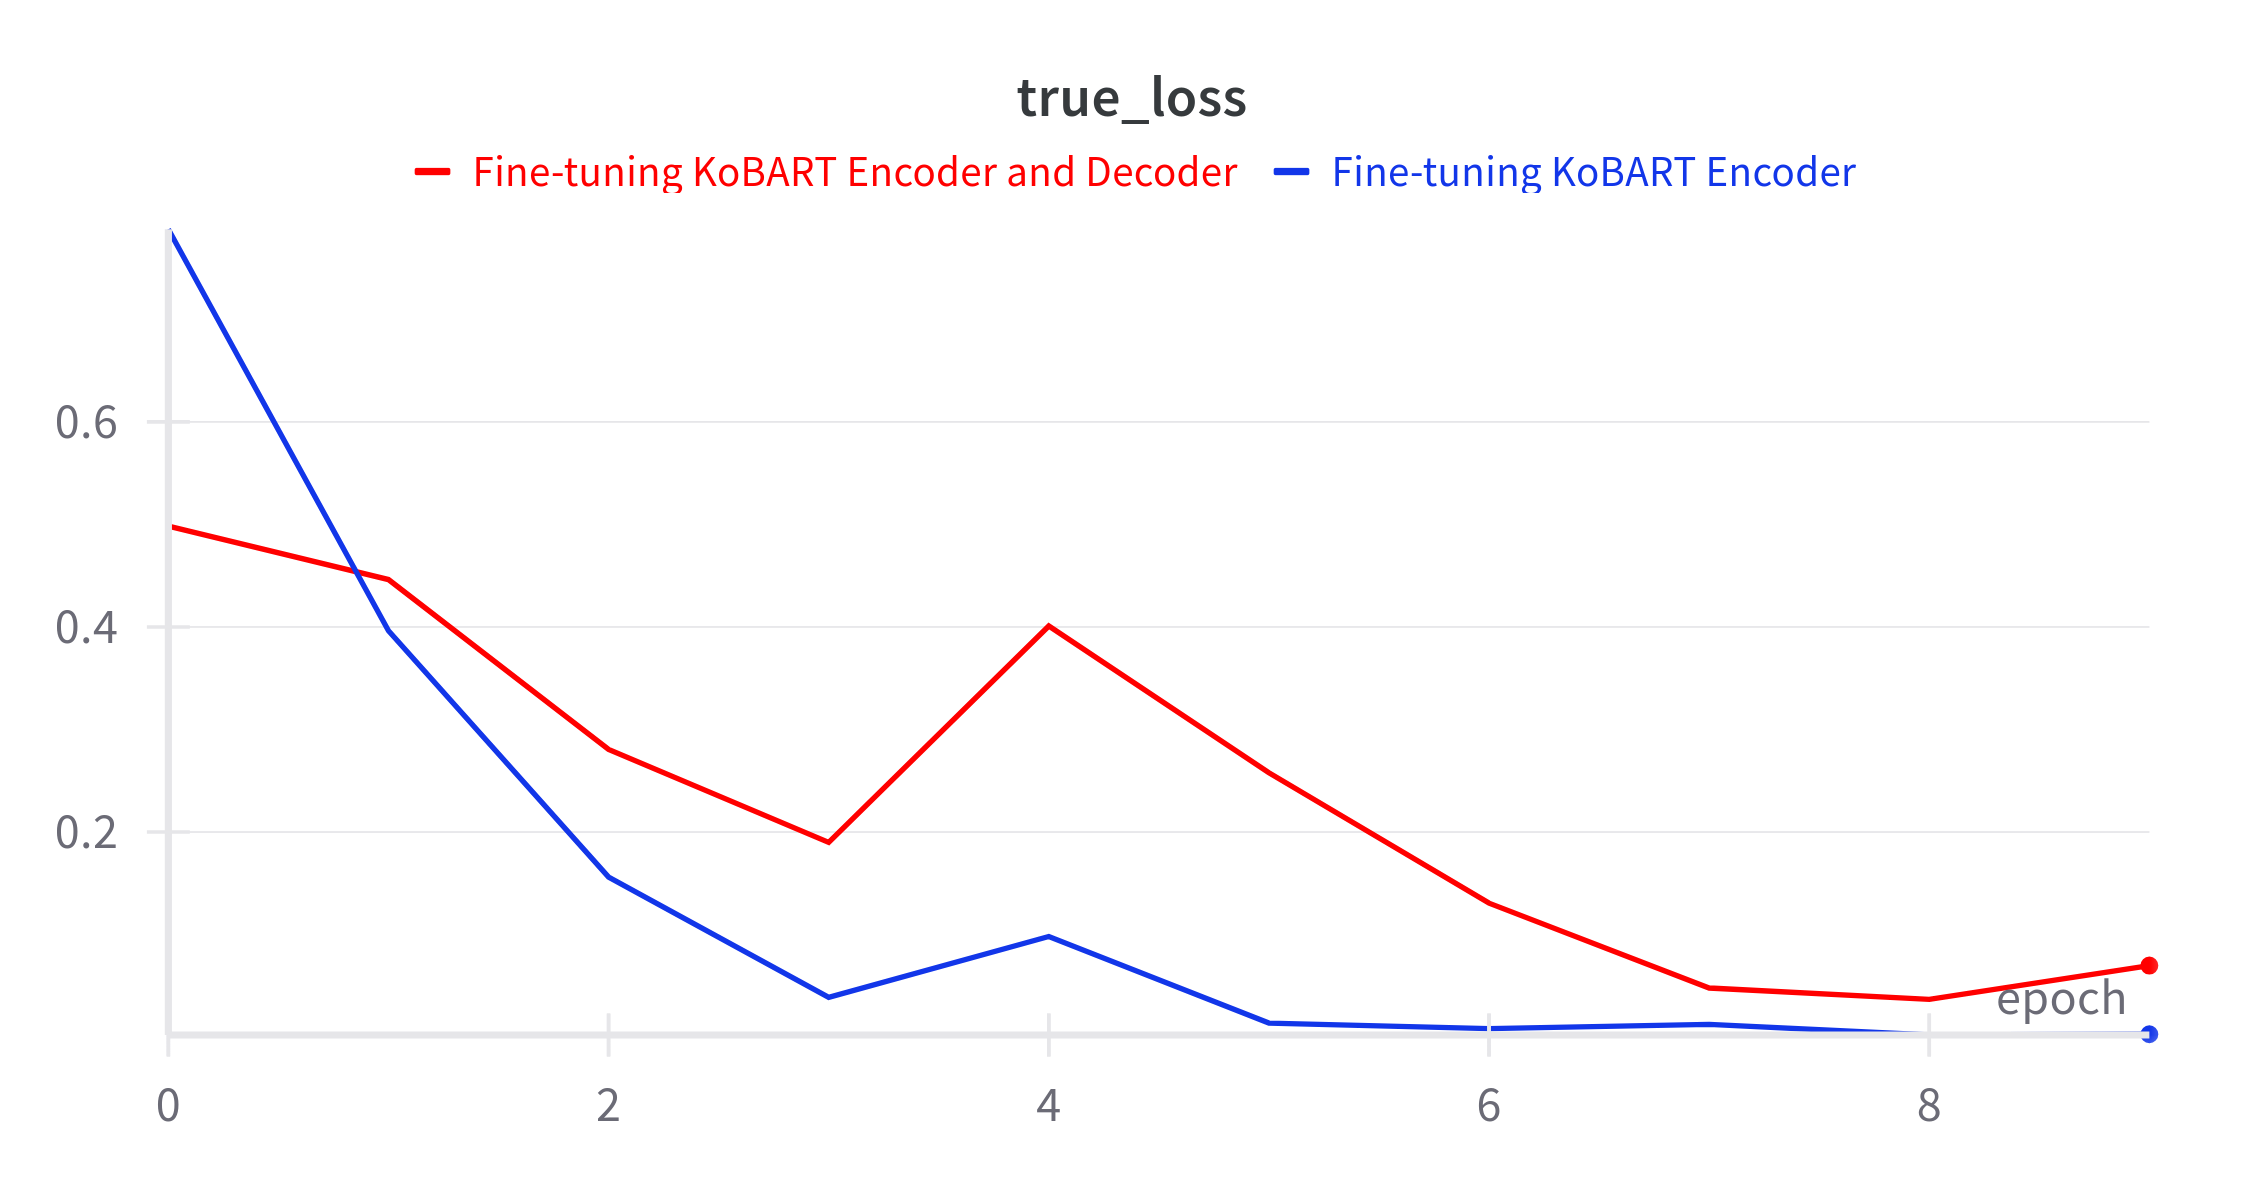
\includegraphics[width=\textwidth]{1_true_loss.png}
        \caption{True Loss}
        \label{fig:acc}
    \end{subfigure}
    \hspace{0.02\textwidth}
    \begin{subfigure}[b]{0.4\textwidth}
        \centering
        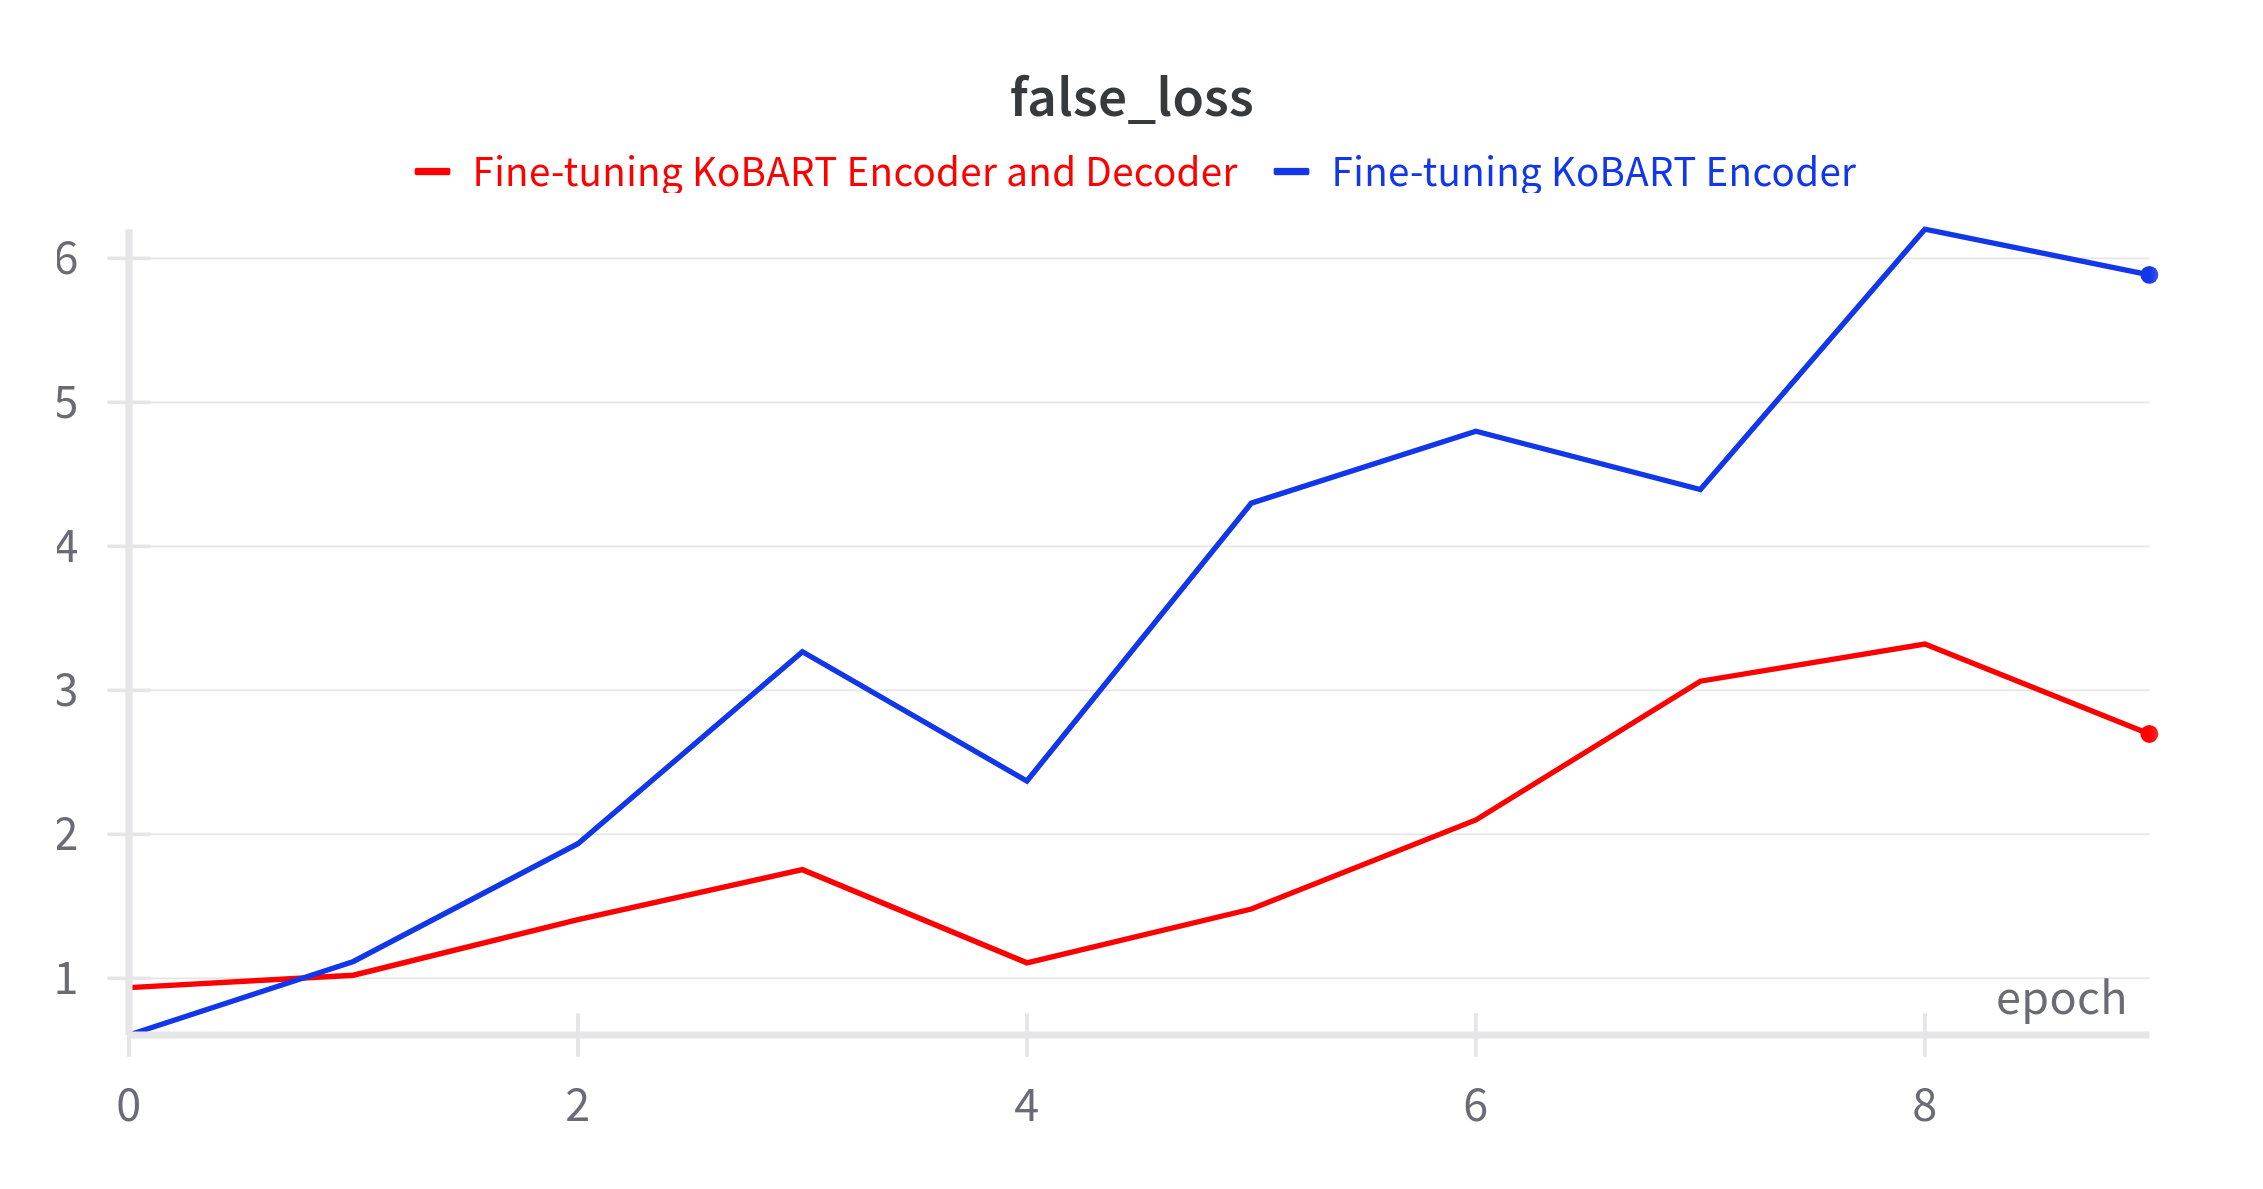
\includegraphics[width=\textwidth]{1_false_loss.png}
        \caption{False Loss}
        \label{fig:loss}
    \end{subfigure}
    
    \vspace{0.4cm}  % 그림 줄 간격 조정
    % 두 번째 줄
    \begin{subfigure}[b]{0.4\textwidth}
        \centering
        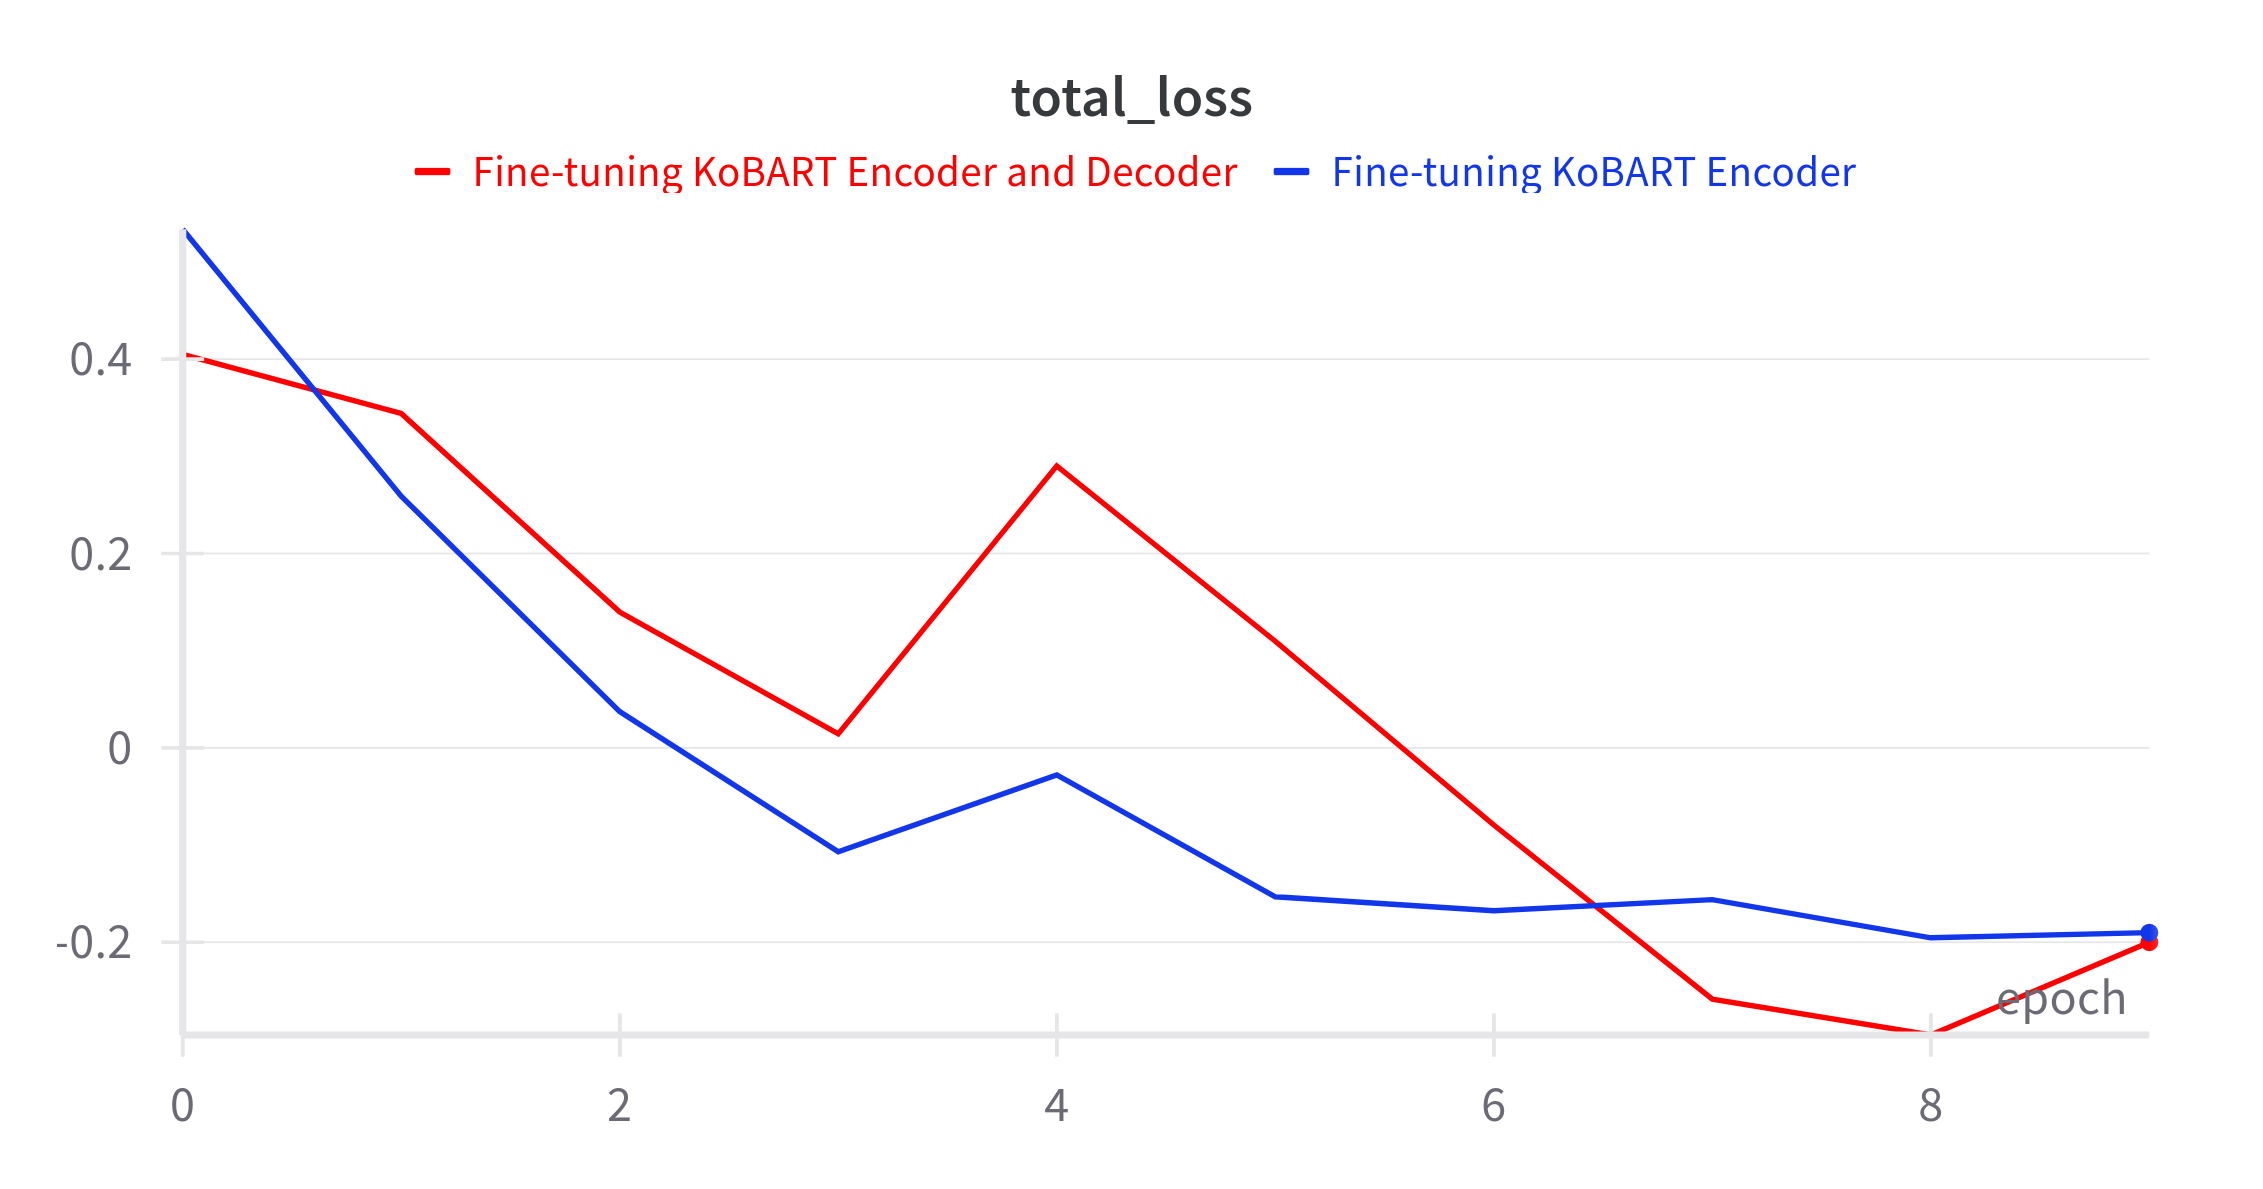
\includegraphics[width=\textwidth]{1_total_loss.png}
        \caption{Total Loss}
        \label{fig:f1}
    \end{subfigure}
    \hspace{0.02\textwidth}
    \begin{subfigure}[b]{0.4\textwidth}
        \centering
        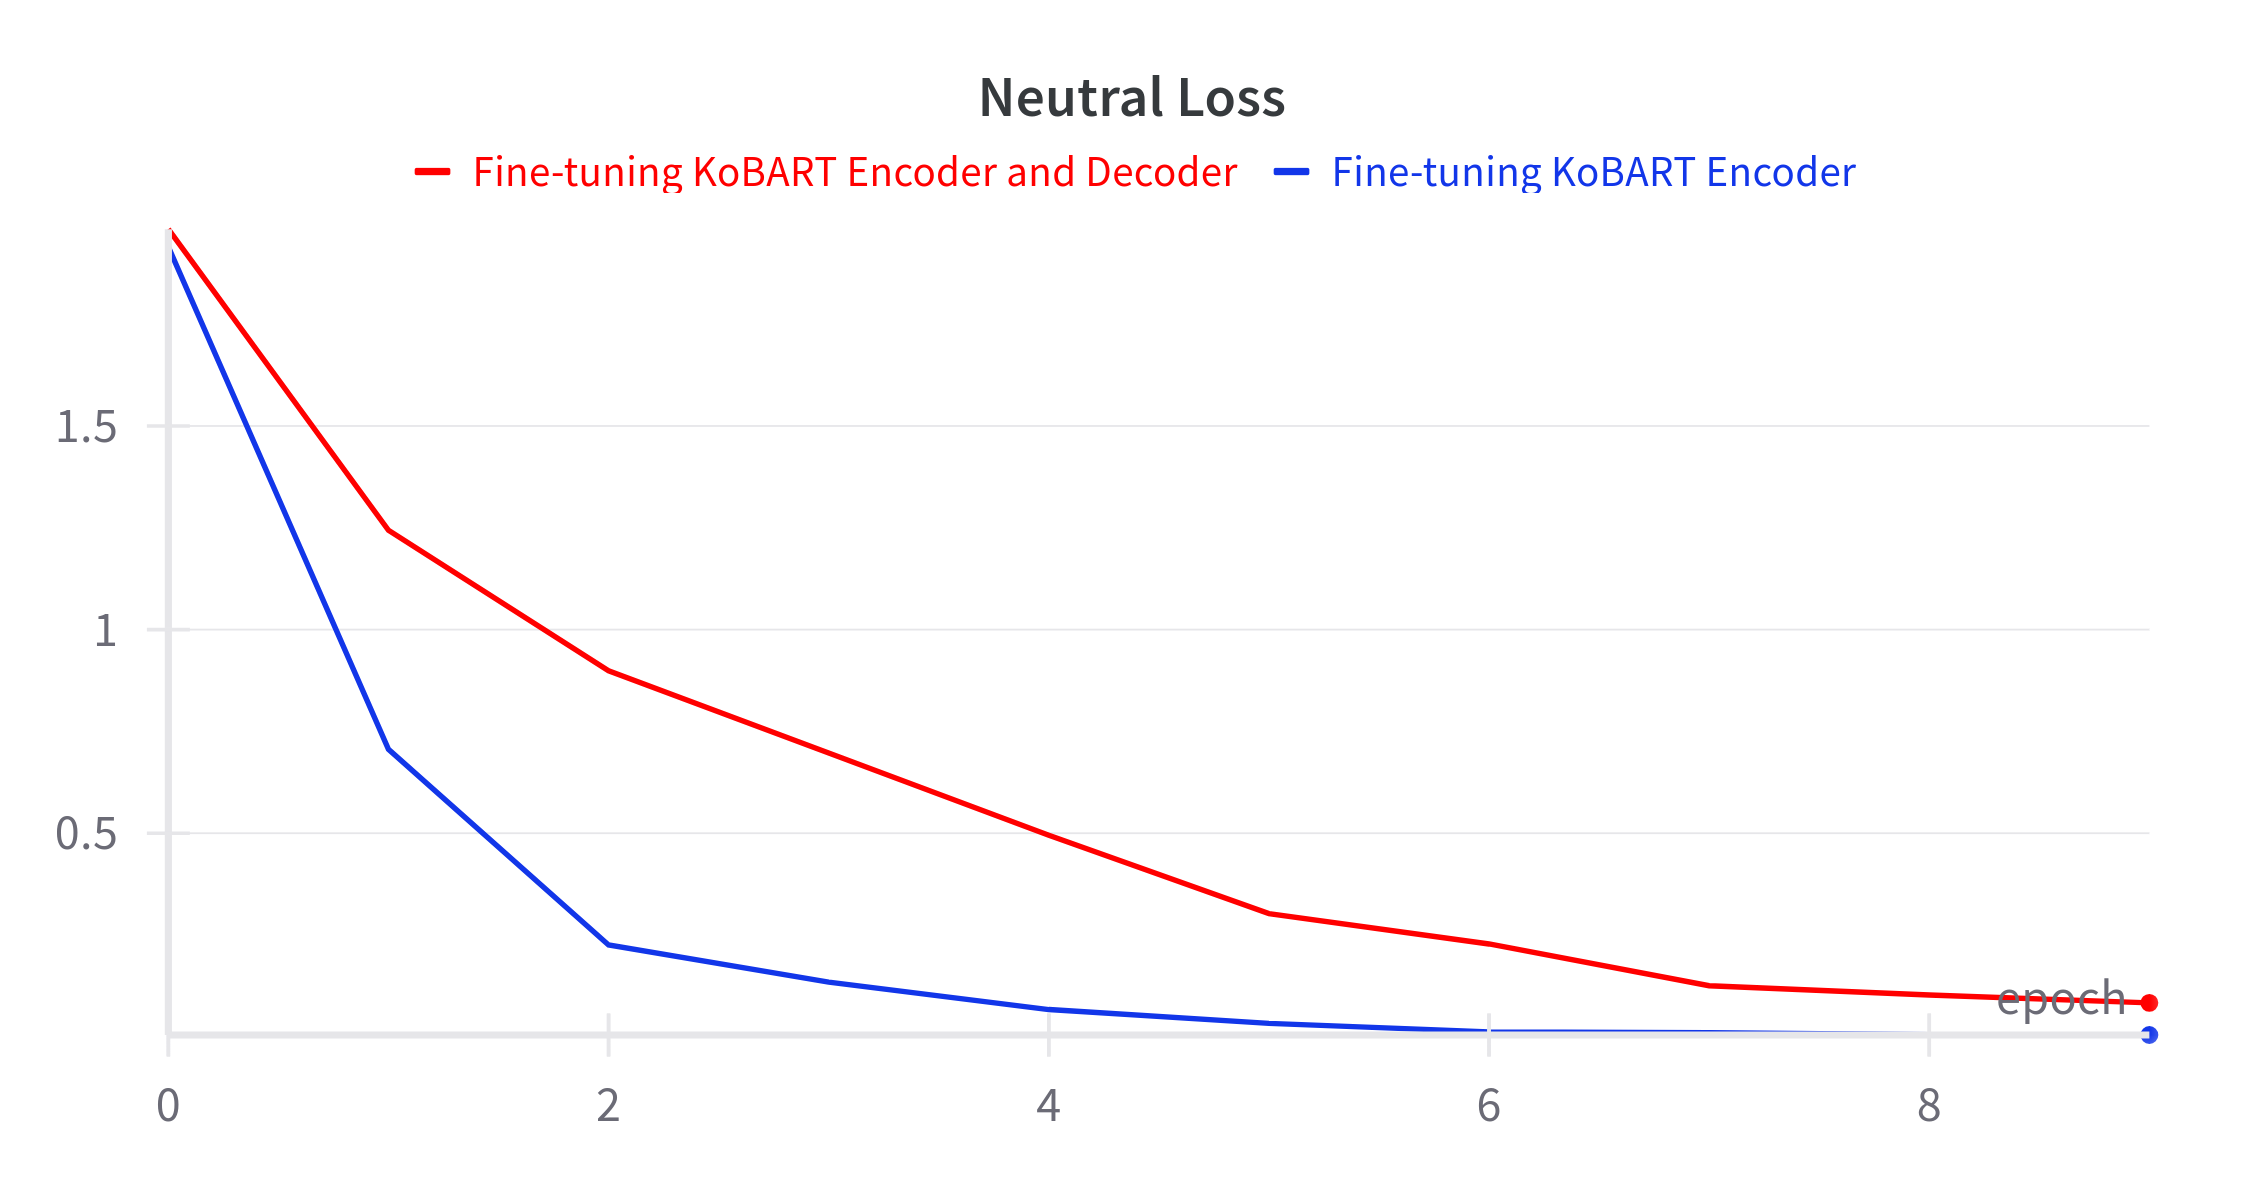
\includegraphics[width=\textwidth]{1_neutral_loss.png}
        \caption{Neutral Loss}
        \label{fig:prec}
    \end{subfigure}
    
    \caption{Decoder 포함 구조와 Encoder-only 구조의 성능 비교}
    \label{fig:performance_grid}
    \end{figure}

   
\subsubsection{Comparison of fine-tuning performance by removing relation types}
\FloatBarrier
관계 기반 Fine-tuning의 효과를 분석하기 위해, neutral 관계 손실과 contradiction 관계 손실을 각각 제거한 ablation 실험을 수행하였다.
그림 4는 각 관계 유형 제거 여부에 따른 학습 성능의 차이를 시각화한 결과로, train loss, accuracy의 변화를 비교하여 보여준다.  
그 결과, neutral loss를 제외한 경우보다 contradiction loss를 제외한 경우에 모델의 Accuracy가 더 크게 감소하는 경향을 보였다.  
특히, 모든 관계 유형을 포함하여 fine-tuning한 설정이 가장 우수한 성능을 보였으며, 이는 neutral 및 contradiction 정보가 서로 보완적으로 작용함을 시사한다.  
또한, contradiction 손실을 제외한 경우가 neutral 손실을 제외한 경우보다 accuracy 하락 폭이 더 컸으며, 이는 contradiction 관계가 모델 업데이트에 보다 중요한 역할을 수행함을 보여준다.

    \begin{figure}[htbp]
        \centering
        \begin{subfigure}[b]{0.48\textwidth}
            \centering
            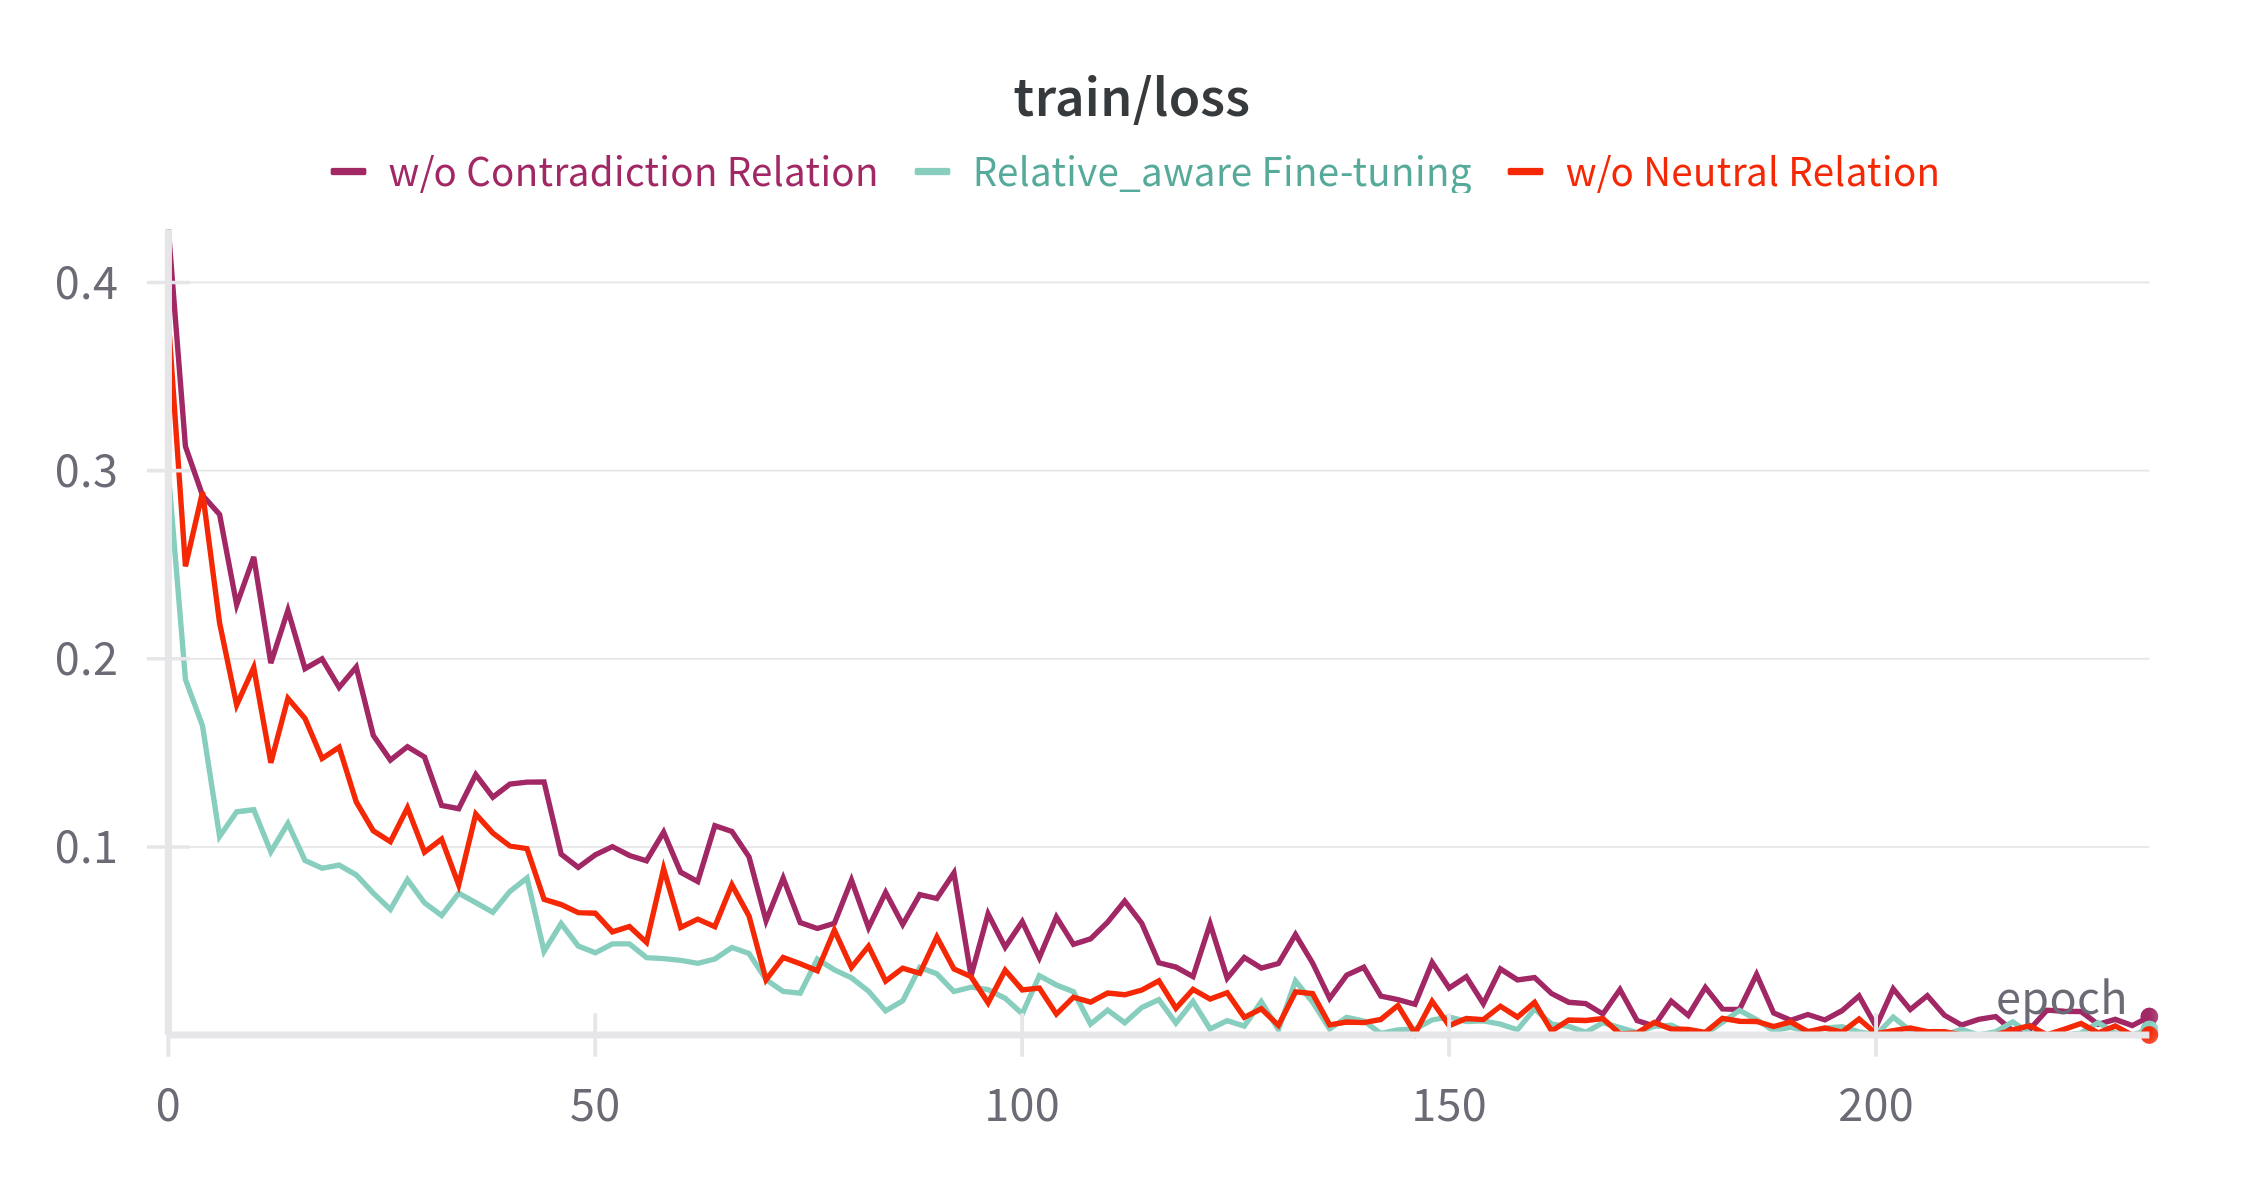
\includegraphics[width=\textwidth]{2_train_loss.png}
            \caption{Train Loss}
            \label{fig:neutral_only}
        \end{subfigure}
        \hspace{0.02\textwidth}
        \begin{subfigure}[b]{0.48\textwidth}
            \centering
            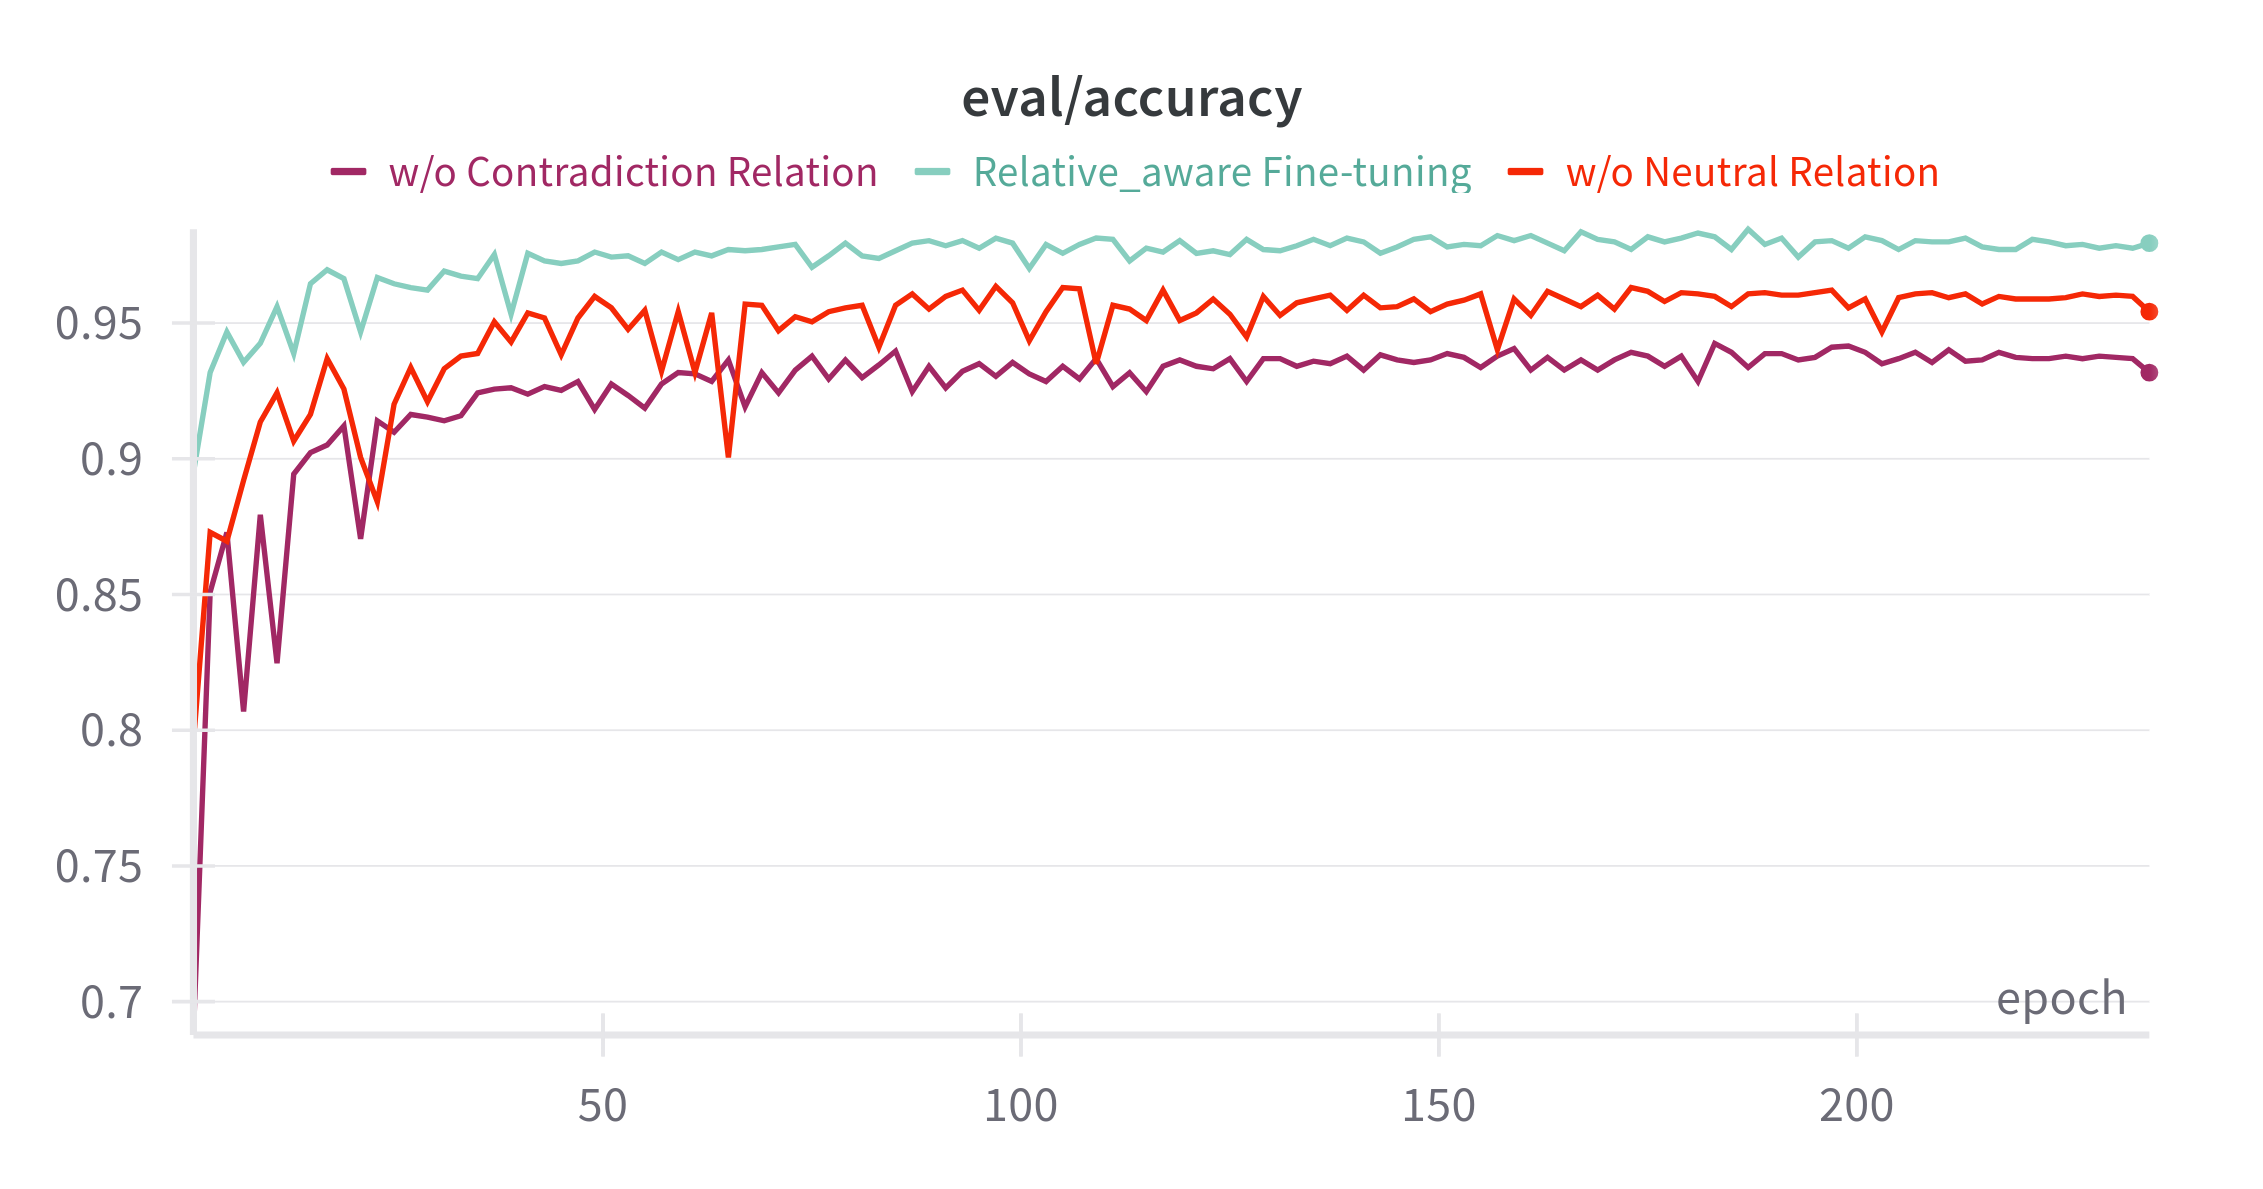
\includegraphics[width=\textwidth]{2_accuracy.png}
            \caption{Accuracy}
            \label{fig:both_relations}
        \end{subfigure}
        \caption{관계 기반 Fine-tuning에서 \texttt{neutral}, \texttt{contradiction} 손실 항목 제거에 따른 모델 성능 변화 비교.}
        \label{fig:relation_ablation}
    \end{figure}
  


\subsubsection{Retrieved data comparison based on the presence of a cross-encoder}

FAISS 기반 벡터 검색은 입력 쿼리와 의미적으로 유사한 문장을 고속으로 반환할 수 있는 효율적인 검색 방식이다. 
그러나 이 방식은 문장 임베딩 간의 L2 거리 또는 코사인 유사도에 의존하기 때문에, 문맥 수준의 정밀한 의미 일치나 논리적 관계성을 충분히 반영하지 못하는 한계가 있다.

이러한 한계를 보완하기 위해 본 연구는 FAISS 검색 결과를 Cross-Encoder 기반 재랭킹 모델에 통과시켜, 쿼리와 검색 문장 간의 의미적 정합성을 더욱 정밀하게 평가하는 절차를 도입하였다. 
Cross-Encoder는 문장 쌍 전체를 입력으로 받아 상호작용을 학습하므로, 단순 벡터 유사도 기반 접근보다 문맥적 일치성과 의미적 일관성을 정밀하게 판별할 수 있다.

실험 결과, Cross-Encoder를 적용한 경우 쿼리 문장의 핵심 의미와 밀접하게 관련된 문장들이 높은 순위로 재정렬되는 경향을 보였으며, 이는 downstream task인 NLI 관계 판단 및 fine-tuning의 정밀도 향상에 기여하였다. 예를 들어, “국내 백신을 해외에 다 빼앗길 판”과 같은 쿼리에 대해, FAISS 단독 검색 결과는 단순한 백신 관련 문장을 반환한 반면, Cross-Encoder는 백신 수급 불균형이나 해외 공급 상황과 직접적으로 관련된 문장을 상위에 위치시켰다.
따라서 Cross-Encoder는 검색 결과의 잡음을 줄이고, 모델 편집의 정확도와 안정성을 높이는 데 필수적인 역할을 수행한다. 
특히, NLI 기반 관계 분류와 선택적 fine-tuning 전략을 채택한 본 시스템에서는 문장 간 정밀한 의미 정합성이 전체 시스템의 품질을 좌우하는 핵심 요소이므로, Cross-Encoder는 선택이 아닌 필수 모듈로 간주된다.

이와 같은 효과는 Table~\ref{tab:retrieval-results}에 제시된 예시를 통해 확인할 수 있다. 
Cross-Encoder를 적용한 경우, 쿼리 문장과 실제로 더 밀접한 의미를 지닌 문장들이 상위에 위치함으로써, 단순 벡터 기반 검색 결과보다 문맥 정합성이 우수한 결과를 제공함을 알 수 있다.

    \renewcommand{\arraystretch}{1.35}
    \begin{table}[H]
    \caption{Cross-Encoder 적용 여부에 따른 Retrieve 문장 비교 예시}
    \label{tab:retrieval-results}
    \centering
    \small
    \begin{tabularx}{\textwidth}{>{\raggedright\arraybackslash}p{3.7cm}X
                                        S[table-format=1.3]
                                        S[table-format=1.3]}
    \toprule
    \textbf{Query} & \textbf{Retrieved Sentence} & \textbf{Sim. Score} & \textbf{Re-rank Score} \\
    \midrule
    
    \multirow{3}{=}{\textbf{국내 백신을 해외에 다 빼앗길 판}} 
    & 백신 개발돼도 해외에 다 뺏길 판…불만 쌓일 대로 쌓였다 & 0.790 & 0.611 \\
    & 백신 선택권이 없어 중국산 백신 맞는다 & 0.781 & 0.400 \\
    & 한국만 백신 선택권이 없다 & 0.772 & 0.312 \\
    \midrule
    
    \multirow{3}{=}{\textbf{불가리스가 코로나19에 효과}} 
    & 불가리스가 코로나 19를 77.8\% 수준으로 억제하는 효과 분석 & 0.812 & 0.730 \\
    & 방역 수준은 에탄올만큼 떨어져 죽는 것으로 추정 & 0.811 & 0.188 \\
    & 노바백스의 코로나19 백신 후불보급 & 0.813 & 0.177 \\
    \midrule
    
    \multirow{3}{=}{\textbf{AZ백신은 국내 허가됨}} 
    & 노바백스 백신은 인허가를 통해 도입 계획임 & 0.867 & 0.433 \\
    & 계약은 비밀유지협약과 함께 진행됨 & 0.847 & 0.358 \\
    & 스푸트니크V 백신 도입 추진 중 & 0.858 & 0.271 \\
    \midrule
    
    \multirow{3}{=}{\textbf{머리카락이 코로나를 옮긴다}} 
    & 머리카락이 신종 코로나 바이러스를 옮긴다 & 0.844 & 0.870 \\
    & 비타민 C를 먹으면 도움이 된다는 주장 & 0.806 & 0.191 \\
    & 마스크 내 화학물질이 폐암 유발할 수 있다 & 0.792 & 0.169 \\
    \bottomrule
    \end{tabularx}
    \end{table}
   

\subsubsection{Performance comparison based on contradiction loss design}

본 연구에서는 모델이 기존 지식을 효과적으로 제거하도록 유도하는 Contradiction Loss의 설계 방식이 전체 학습 성능에 미치는 영향을 비교하였다. 이를 위해 총 네 가지 손실 함수 조합을 설정하였으며, 각 방식은 \ref{tab:loss-designs}에 정리되어 있다.
\begin{table}[H]
    \centering
    \renewcommand{\arraystretch}{1.3}
    \caption{Contradiction Loss 구성 방식별 총합 손실 함수 정의}
    \label{tab:loss-designs}
    \begin{tabularx}{\textwidth}{>{\raggedright\arraybackslash}p{1.2cm}X}
        \toprule
        \textbf{Case} & \textbf{Total Loss 정의} \\
        \midrule
        (1) & \( \mathcal{L} = \log(\text{True Loss}) + \log(\text{False Loss}) \) \\
        (2) & \( \mathcal{L} = \log(\text{True Loss}) - \log(\text{False Loss}) \) \\
        (3) & \( \mathcal{L} = \log(\text{True Loss}) - \alpha \cdot \log(\text{False Loss}) \quad (\alpha = 0.5) \)\\
        (4) & \( \mathcal{L} = \log(\text{True Loss}) - \alpha \cdot \log(\text{False Loss}) \quad (\alpha = 0.1) \) \\
        \bottomrule
    \end{tabularx}
\end{table}
   
실험 결과는 다음과 같다.
\begin{itemize}
    \item \textbf{Case (1)}의 경우, False Loss가 학습이 진행됨에 따라 오히려 감소하는 현상이 관찰되었으며, 이는 모델이 contradiction 관계에 대해 역으로 보존하려는 경향을 보임을 시사한다.
    
    \item \textbf{Case (2)}와 \textbf{(3)}에서는 False Loss의 영향력이 과도하게 커져 Total Loss가 음수로 수렴하며, True Loss는 학습 초기에 0 부근에서 정체되어 더 이상 감소하지 않는 문제가 발생하였다.
    
    \item \textbf{Case (4)}는 \(\alpha = 0.1\)을 적용한 방식으로, True Loss는 안정적으로 감소하고 False Loss는 점진적으로 증가하는 이상적인 손실 곡선을 보였다.
\end{itemize}
    
결론적으로, contradiction 관계를 반영하는 데 있어 False Loss의 기여도를 적절히 조정하는 것이 중요하며, 본 연구에서는 \(\alpha = 0.1\) 설정이 가장 안정적인 학습 성능을 보여주었다.

\begin{figure}[htbp]
    \centering

    \begin{subfigure}[b]{0.48\textwidth}
        \centering
        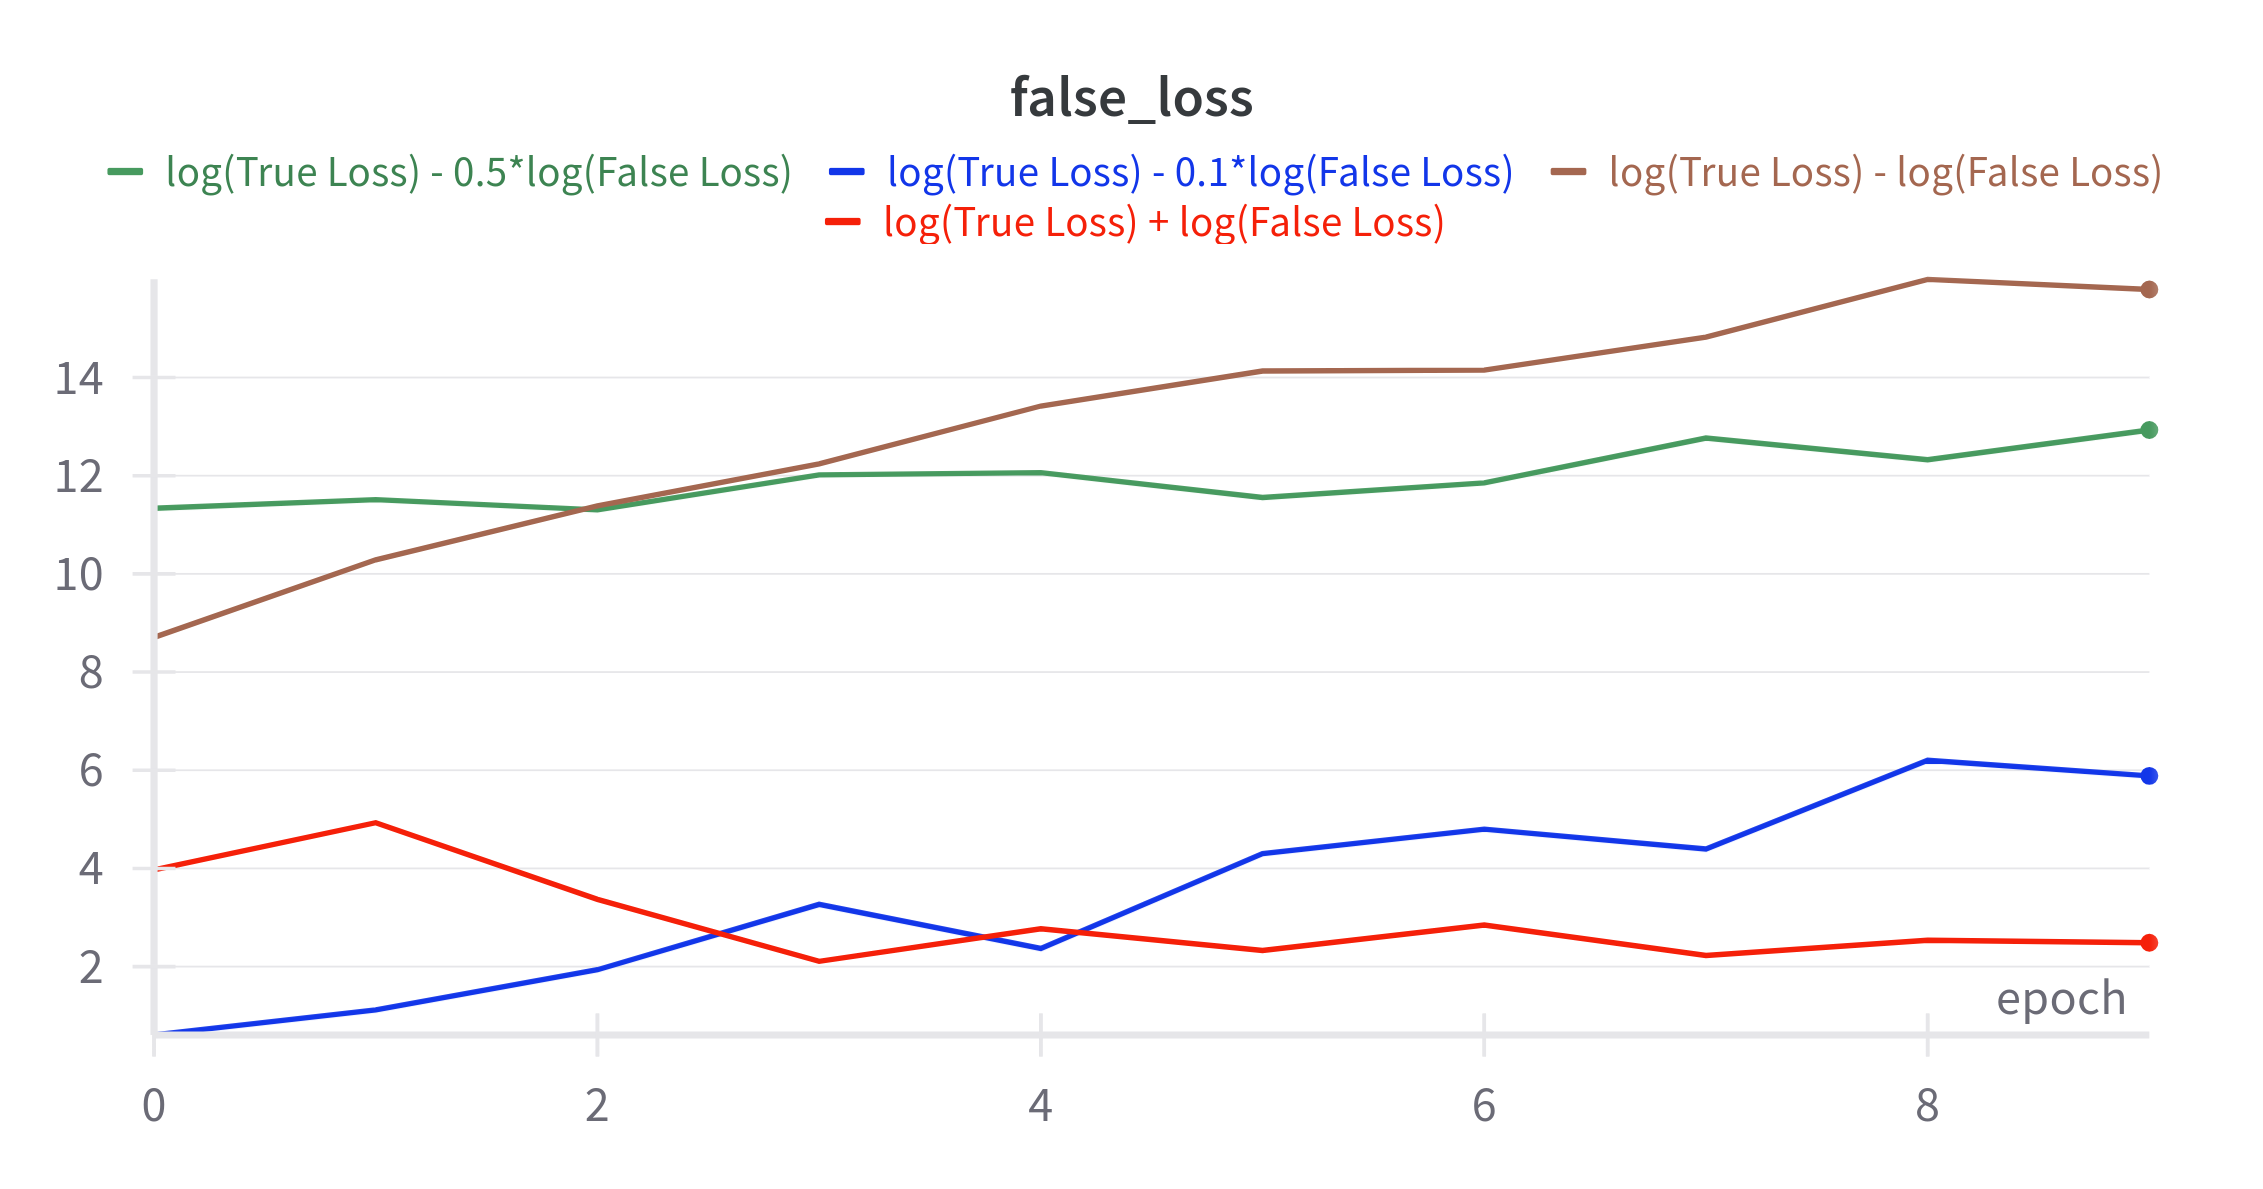
\includegraphics[width=\textwidth]{3_false_loss.png}
        \caption{Train Loss}
        \label{fig:neutral_only}
    \end{subfigure}
    \hspace{0.02\textwidth}
    \begin{subfigure}[b]{0.48\textwidth}
        \centering
        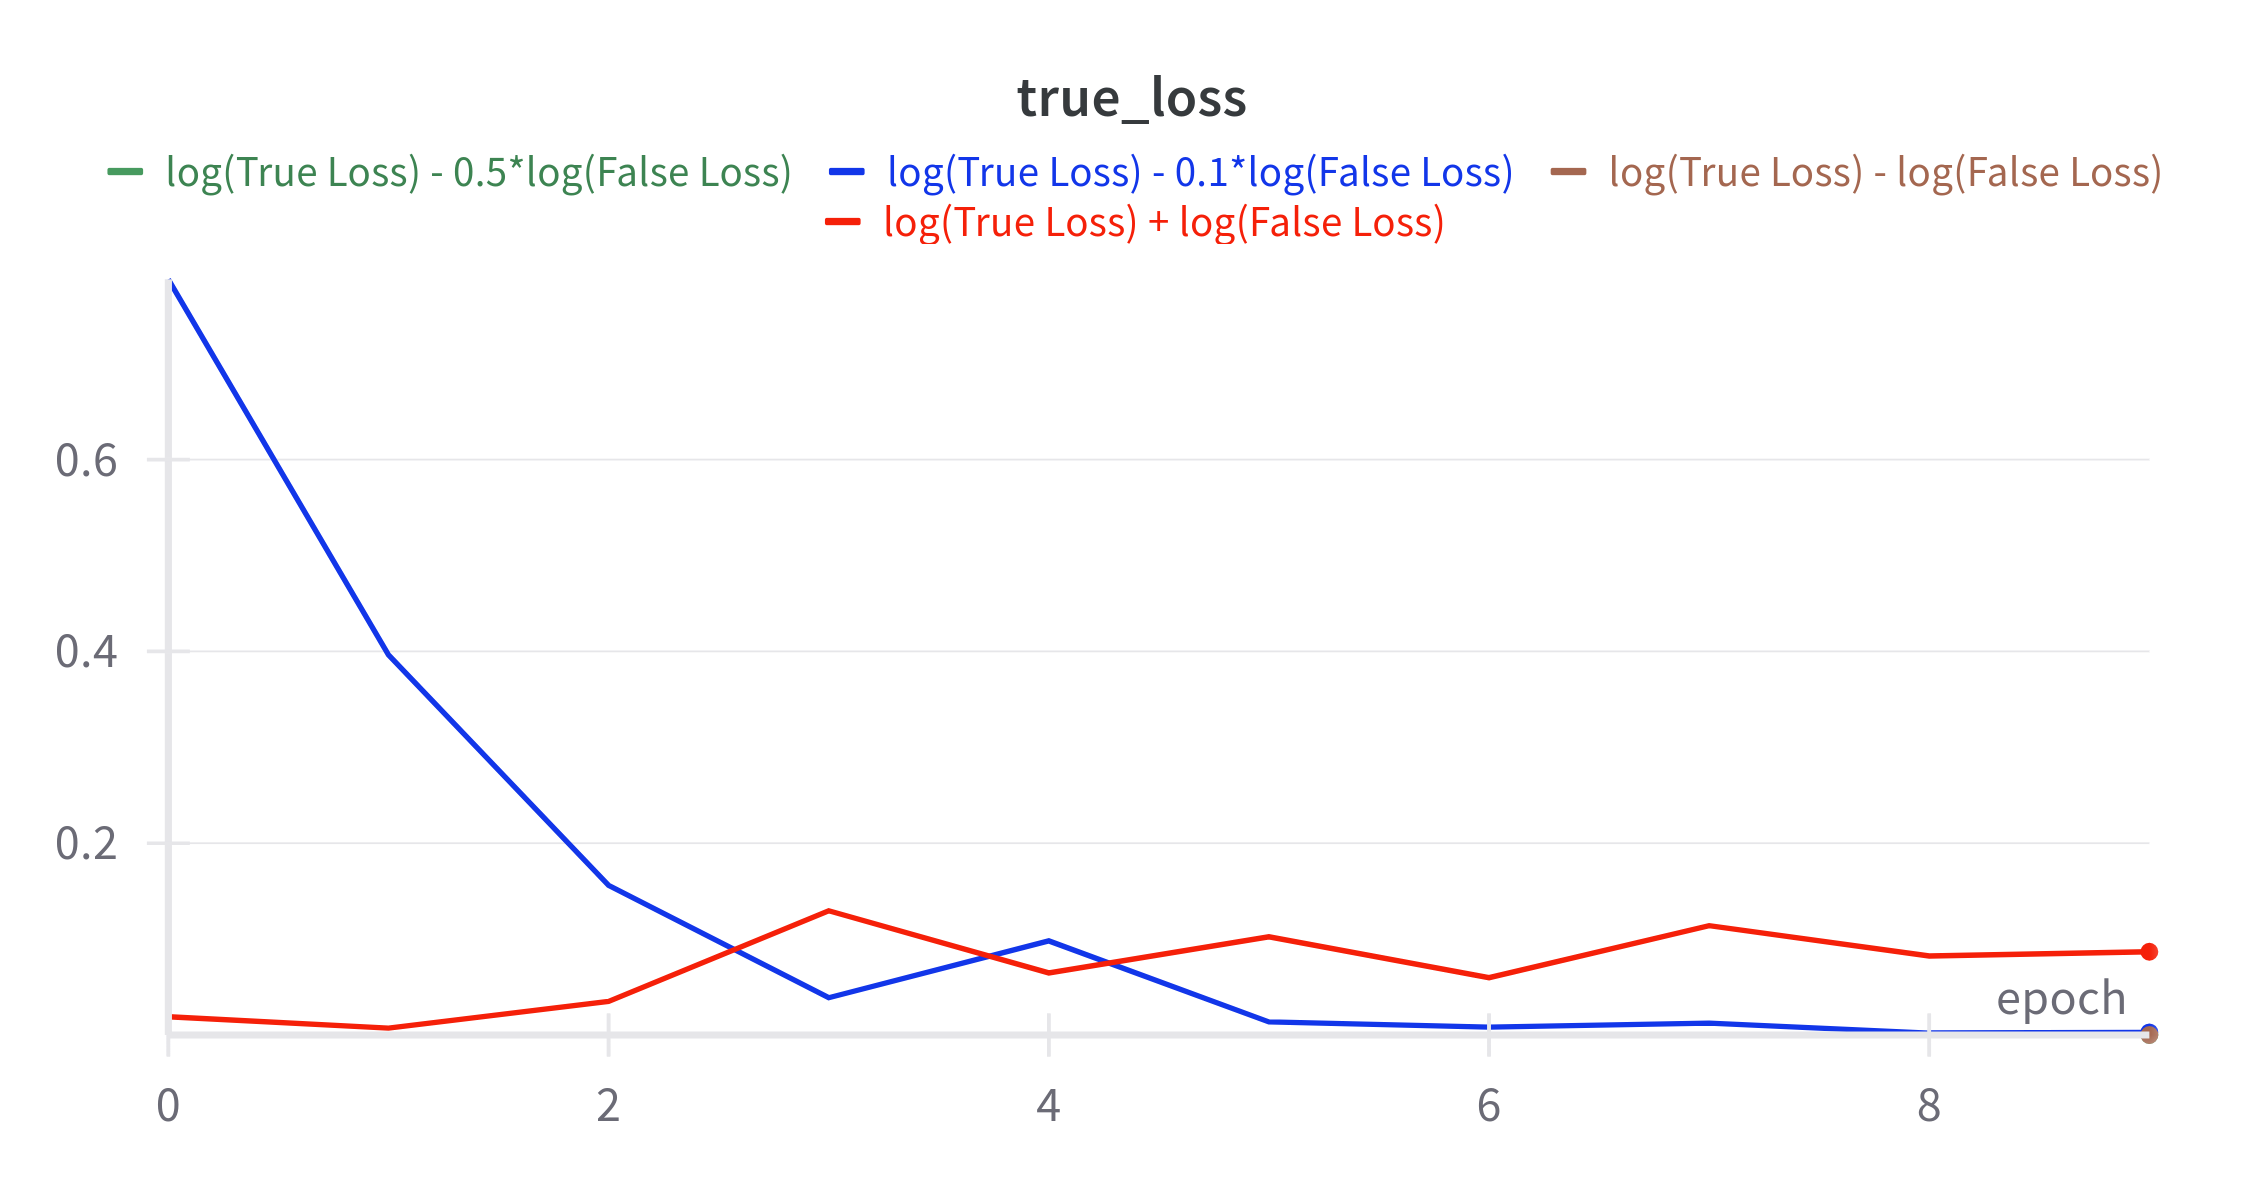
\includegraphics[width=\textwidth]{3_true_loss.png}
        \caption{Accuracy}
        \label{fig:both_relations}
    \end{subfigure}
    \hspace{0.02\textwidth}
    \begin{subfigure}[b]{0.48\textwidth}
        \centering
        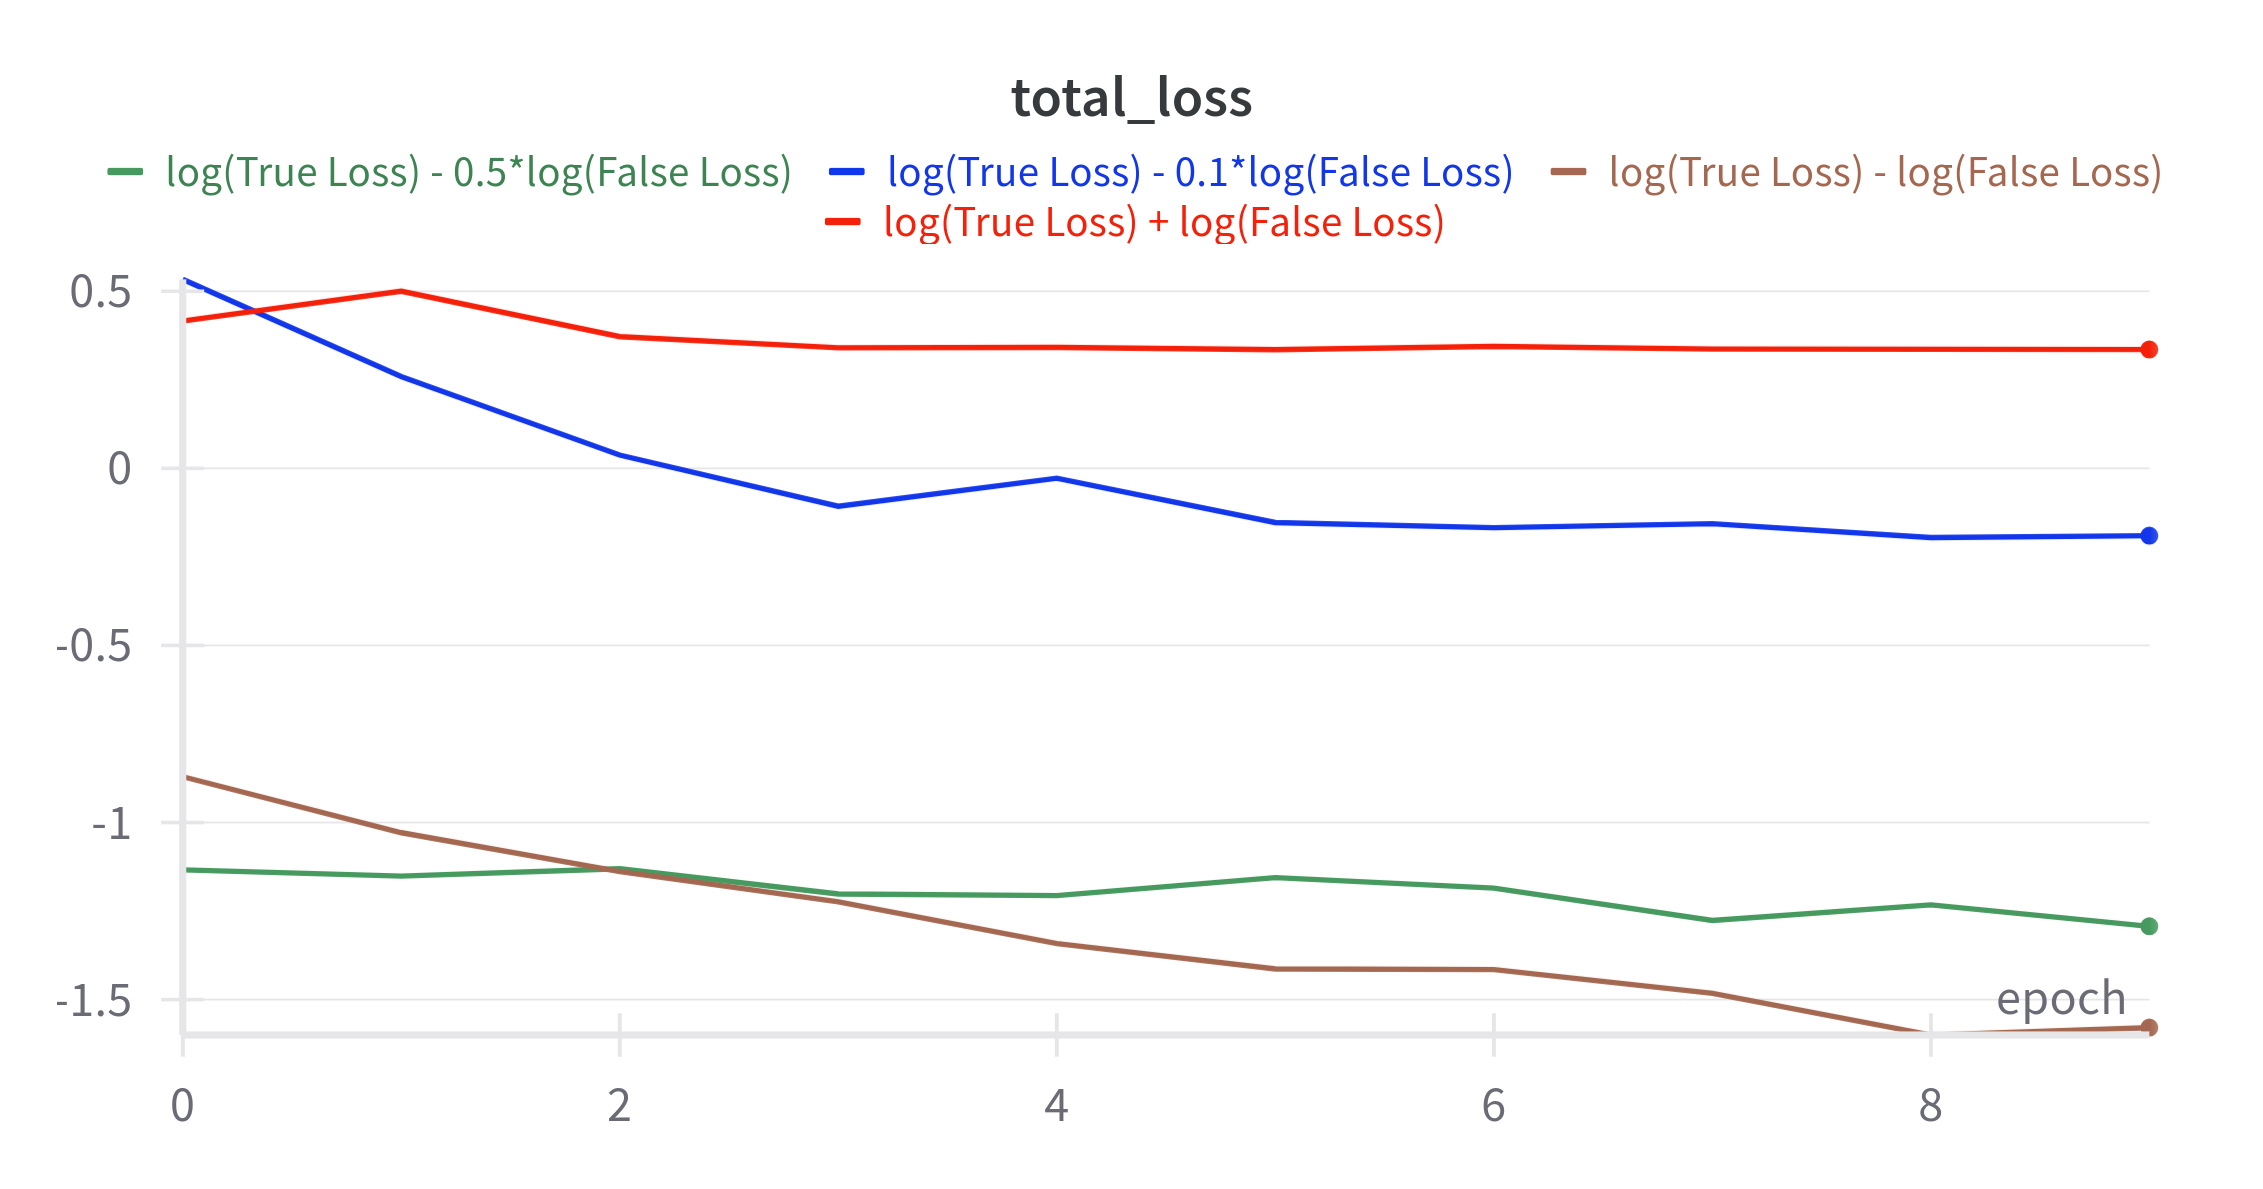
\includegraphics[width=\textwidth]{3_total_loss.png}
        \caption{Accuracy}
        \label{fig:both_relations}
    \end{subfigure}
    \caption{contradiction loss 설계에 따른 성능어떤 걸 써야 학습이 되는가에 대한 비교}
    \label{fig:relation_ablation}
\end{figure}

\subsubsection{Comparative analysis of encoder fine-tuning strategies}

\subsection{Performance Comparison}
\subsubsection{Performance comparison by dataset configuration}

기존의 일반적인 fine-tuning 방식과

본 연구에서 제안한 Relation-aware Fine-Tuning 방식을 동일한 모델(KoBART) 기반으로 비교하여 성능 우위를 입증

Plain Fine-Tuning	전체 학습 데이터를 사용하여 한 번에 fine-tuning 수행. 관계 판단 없음.
Selective Relation-based Fine-Tuning	NLI 기반으로 관계를 판단하여 entailment는 제외하고, contradiction 및 neutral 관계만 fine-tuning 수행

\begin{table}[htbp]
    \centering
    \caption{Dataset configurations for transfer learning.}
    \resizebox{\textwidth}{!}{%
    \begin{tabular}{lcccc}
    \toprule
    \textbf{Datasets} & \textbf{Test 1} & \textbf{Test 2} & \textbf{Test 3} & \textbf{Test 4} \\
    \midrule
    Pretraining & Old data(2019 from Kaggle)
             & +New data(Training)
             & +AI FactChecknet(Transfer data)
             & -Old data(2019 from Kaggle) \\
   
    \bottomrule
    \end{tabular}%
    }
    \end{table}
    
초록색은 eval loss 발산
pretrain data에 따른 정확도(dataset configuration에 따른 성능)


기존 baseline (no retrieval / no NLI)

제안 모델과의 성능 비교


encoder의 MLP만 Fine-tuning하는 이유 -> all parater tuning과 encoder MLP만 학습했을 때 성능 비교(별 차이없음)

Locality 평가는 모델이 편집되지 않은 입력에 대해 기존 출력 동작을 얼마나 유지하는지를 측정하기 위해 수행되었다. 이를 위해 COVID-19 쿼리 문장 100개에 대해 각 쿼리당 의미적으로 무관한 문장 5개씩, 총 500개의 샘플을 AI FactCheckNet으로부터 수집하였다. 이 데이터는 보건, 정치, 경제, 사회 등 다양한 분야의 팩트체크 문장으로 구성되어 있으며, COVID-19 관련 문장은 포함되어 있지 않다. 따라서 해당 문장들은 모델이 fine-tuning을 통해 편집한 내용과 주제적, 의미적으로 명확히 분리되어 있다고 판단할 수 있다.

모델 편집 전과 후의 예측 결과를 비교한 결과, 전체 500개 중 470개의 문장에서 동일한 예측 결과가 유지되어 약 94.0의 Locality를 달성하였다. 이는 Relation-aware Fine-tuning이 편집되지 않은 입력에 대한 모델의 동작을 대부분 유지하면서도, 필요 시 정확한 편집이 이루어졌음을 의미한다. 본 결과는 기존 연구인 ROME이 보고한 96.8% 수준의 Locality에 근접하며, 제안한 접근법이 LLM 편집의 안정성 측면에서도 효과적임을 보여준다
%---------------------------------------------------

본 절에서는 제안한 Relation-aware Fine-tuning 모델과 기존 베이스라인 모델 간의 성능을 비교하고, 파라미터 업데이트 방식에 따른 효율성을 분석하였다.

우선, Locality 평가는 모델이 편집되지 않은 입력에 대해 기존 출력 동작을 얼마나 잘 유지하는지를 측정하기 위해 수행되었다. 이를 위해 COVID-19 관련 쿼리 문장 100개를 선정하고, 각 쿼리당 의미적으로 무관한 문장 5개씩 총 500개의 샘플을 AI FactCheckNet으로부터 수집하였다. 이 데이터는 정치, 경제, 사회, 문화 등 다양한 주제를 포함하지만 COVID-19 관련 문장은 포함되어 있지 않다. 따라서 이들은 모델이 fine-tuning을 통해 편집한 쿼리와 주제적으로 명확히 분리되어 있는 샘플이라 할 수 있다.

모델 편집 전후의 예측 결과를 비교한 결과, 전체 500개 중 470개 문장에서 동일한 예측이 유지되어 약 94.0\%의 Locality를 달성하였다. 이는 Relation-aware Fine-tuning이 편집되지 않은 입력에 대해서는 기존 모델의 동작을 안정적으로 유지하면서, 필요한 경우에는 정확하게 지식을 수정할 수 있음을 보여준다. 본 결과는 기존 연구인 ROME이 보고한 96.8\% 수준의 Locality에 근접하며, 제안한 접근법이 안정성과 정합성 측면에서 경쟁력을 갖추고 있음을 시사한다.

또한 본 연구는 다음과 같은 두 가지 베이스라인과 비교 실험을 수행하였다.
\begin{itemize}
    \item \textbf{Baseline 1 (No Retrieval)}: 외부 문서 검색 없이 쿼리 입력만으로 fine-tuning을 수행
    \item \textbf{Baseline 2 (No NLI)}: 검색은 수행하되 Old data와 New data 간의 관계를 고려하지 않고, 무조건 fine-tuning을 수행
\end{itemize}

제안 모델은 Accuracy와 F1 Score 측면에서 두 베이스라인 대비 우수한 성능을 기록하였다. 특히 Contradiction 관계에 대해서만 selective하게 fine-tuning을 수행함으로써, 불필요한 업데이트를 방지하고 모델의 정합성을 유지할 수 있었다.

추가적으로, 전체 모델 파라미터를 fine-tuning하는 방식과 encoder의 MLP 계층만을 fine-tuning하는 방식 간의 성능도 비교하였다. 실험 결과, 두 방식 간의 최종 분류 성능 차이는 유의미하지 않았으며, encoder의 MLP 계층만을 업데이트하는 방식이 연산 자원과 학습 시간을 절감하면서도 유사한 성능을 달성하였다. 이에 따라 본 연구는 효율성과 실용성을 고려하여 encoder의 MLP 계층만을 selective하게 업데이트하는 경량화 전략을 채택하였다.
\subsubsection{Performance comparison: standard vs. relation-aware fine-tuning}

\subsubsection{Evaluation of locality and generality}

\section{Discussion}

\section{Conclusions}

본 연구에서는 COVID-19 관련 허위 정보를 식별하기 위한 모델 편집 기반 접근법으로서, 외부 지식 검색 및 관계 분류 정보를 결합한 \textbf{Relation-aware Fine-Tuning} 프레임워크를 제안했다.  
FAISS 기반 벡터 검색과 Cross-Encoder 재랭킹, 그리고 NLI 기반 관계 판단을 통해, 모델이 기존 지식을 유지하면서도 새로운 정보에 기반한 선택적 업데이트를 수행할 수 있도록 설계하였다.
  
실험 결과, 제안한 Relation-aware Fine-Tuning은 기존 fine-tuning 방식에 비해 더 높은 정확도와 더 우수한 Locality/Generality를 달성하였다.  
특히, Cross-Encoder 기반 재랭킹을 통한 정밀한 문장 선택과, NLI 관계 기반 selective fine-tuning 전략은 모델의 신뢰도와 안정성을 동시에 향상시켰다.  
또한 Contradiction Loss의 구성 방식에 따라 성능이 크게 달라지는 것을 확인하였고, 적절한 가중치 조정(\(\alpha = 0.1\))이 효과적인 학습에 핵심적임을 입증하였다.
  
제안한 방법은 소규모 최신 데이터 기반 모델 수정이 가능하며, 기존 지식의 유지(Locality)를 보장하면서도 새로운 정보 반영 능력(Generality)을 높일 수 있다는 강점을 가진다.  
또한 복잡한 재학습 없이, 특정 문장 단위 지식만 국소적으로 수정하는 구조는 실제 응용 가능성이 높다.  
그러나 NLI 모델 및 Cross-Encoder의 정확도에 따라 전체 시스템 성능이 의존하며, 관계 분류 오류가 fine-tuning 품질에 영향을 줄 수 있다는 한계를 가진다.

  
본 연구는 다음과 같은 방향으로 확장될 수 있다:
\begin{itemize}
    \item \textbf{다른 도메인 적용:} 해양, 기후, 정치 등 다양한 주제의 허위 정보 탐지에 Relation-aware Fine-Tuning을 적용할 수 있다.
    \item \textbf{대형 언어 모델(LLM) 접목:} BART 외에도 LLaMA, GPT 등 대형 사전학습 모델과의 결합을 통해 확장성과 일반화 능력을 높일 수 있다.
    \item \textbf{Knowledge Editing 자동화:} RAG 시스템과 NLI 평가 구조를 통합하여, 사람 개입 없이 자동으로 지식을 수정하고 유지하는 방향으로 발전시킬 수 있다.
\end{itemize}
\clearpage

\printcredits


%\bibliographystyle{cas-model2-names}
%\bibliography{}


\end{document}
